\chapter{Experimentation and Results}


Over the course of this work it was concluded that the radar data was not appropriate for Map Building or for localization using \ac{AMCL}. However it was noted that the radar was quicker   at detecting different types of obstacles. 
With the configuration described in the previous section we can now start to experiment with the robotic platform to do certain navigation tasks. In this part we propose various experiments that try to evaluate the  performance of the \ac{FMCW} \ac{radar} as an alternative or support to the \ac{LiDAR} as an obstacle detector for indoor navigation.




\section {Static Obstacles in controlled environment}
In this work the \ac{FMCW} radar has shown to have better performance at detecting certain indoor objects than the 2D \ac{LiDAR}. This means that there might be situations where using it for obstacle avoidance produce better results for indoor navigation tasks. \\

To demonstrate this a test was devised in a controlled environment that compares the performance of each sensor for different types of obstacles, in this case two types of chairs, a garbage bin, a low height box, a transparent acrylic tube and finally a robot (in this case another tutlebot2).  
%We also try to use the fusion of both sensors that in theory should produce the best results. 
To ensure the experiment is done in a controlled way the scenario shown in Figure \ref{fig:cenario} was constructed. 
\begin{figure}[ht!] 
    \begin{minipage}[t]{.49\linewidth}
        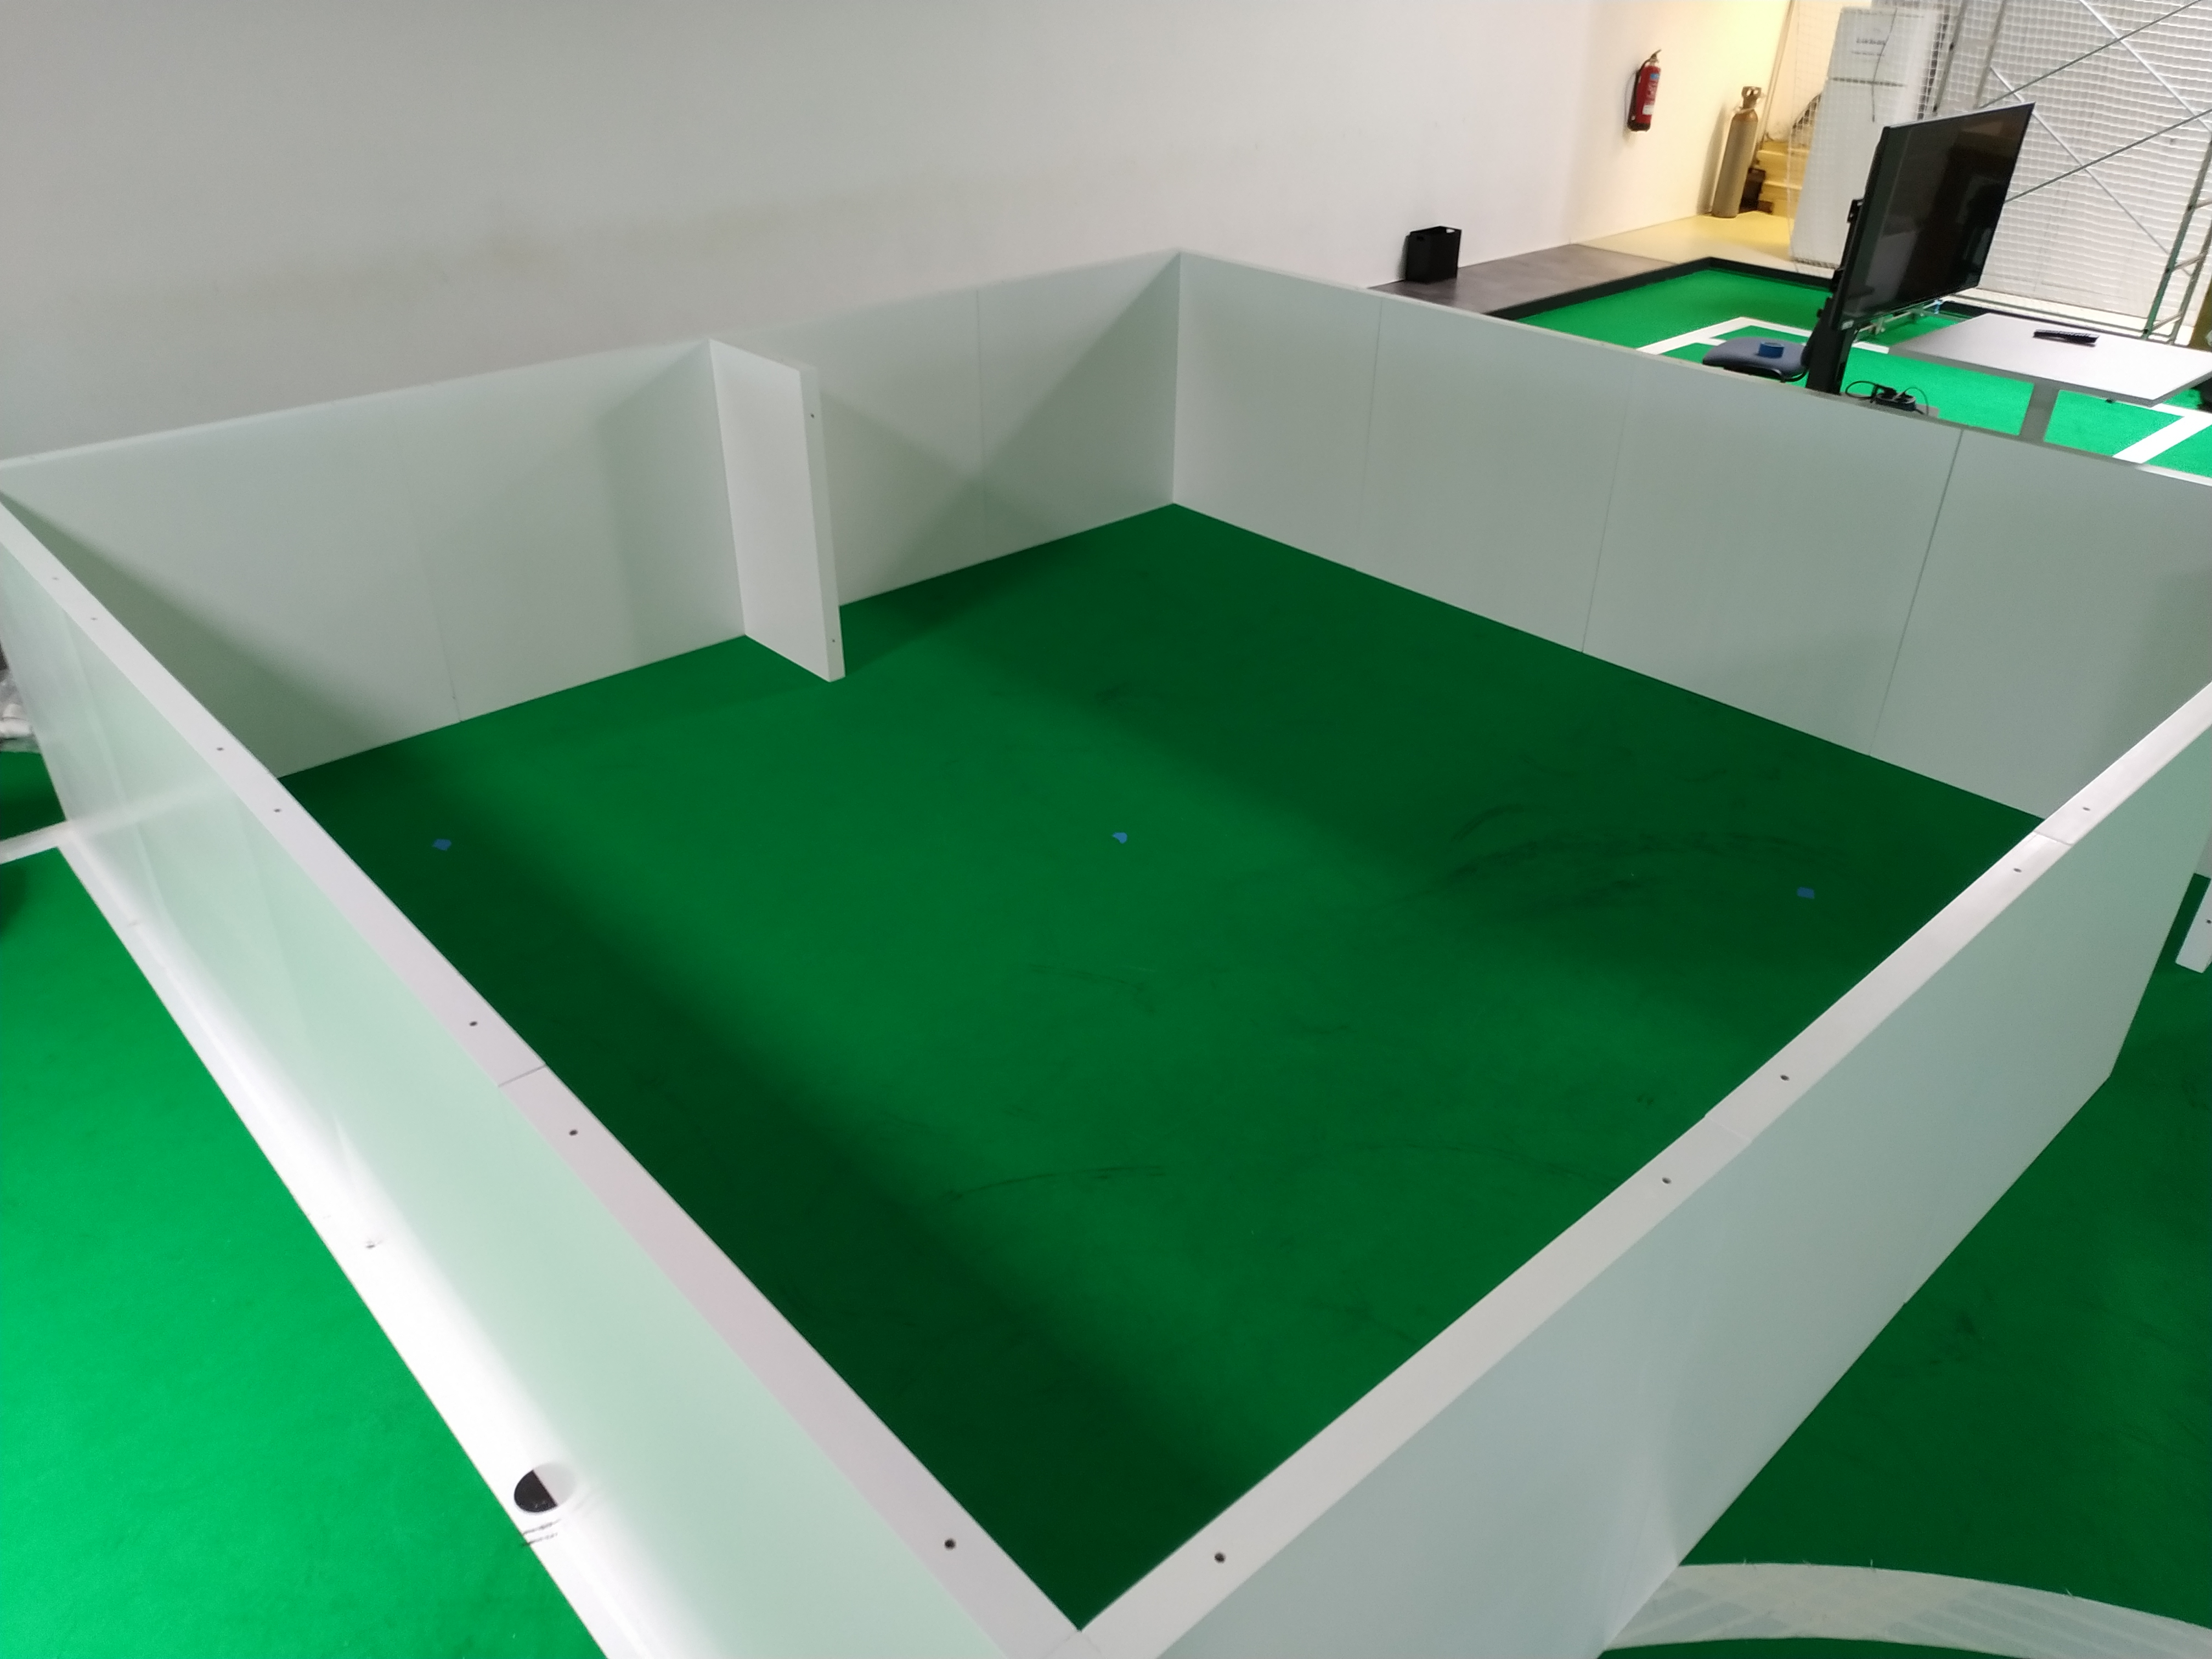
\includegraphics[height=5cm,width=\linewidth]{imgs/chapter5/mapP.jpg}
        \subcaption{Foto of the scenario \cite{robot1}}
        \label{fig:cenario}
    \end{minipage}
    \begin{minipage}[t]{.49\linewidth}
        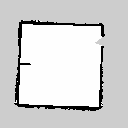
\includegraphics[height=5cm,width=\linewidth]{imgs/chapter5/map.png}
        \subcaption{Map created using \texttt{SLAM} package developed at \ac{IRIS}}
        \label{fig:map}
    \end{minipage}
    \caption{Scenario Constructed for the experiment}
    \label{fig:setup2}
\end{figure}
This is a 4 by 4 meter squared box with 1 meter high walls with the addition of a half a meter wall in length in the middle. This type of environment optimizes the robots localization system (\ac{AMCL}) as well as make sure we only concentrate with one specific object at a time. Using a \texttt{\ac{SLAM}} package developed here at \ac{IRIS} a map is first created (Figure \ref{fig:map}) that will later be used for localization purposes.

\subsection{Experimental setup}
With the described scenario we setup the robots goal to make five loops between two goals, position A and B, positioning in between the route an obstacle as illustrated in  Figure \ref{fig:exp}. 
\begin{figure}[ht!]
\centerline{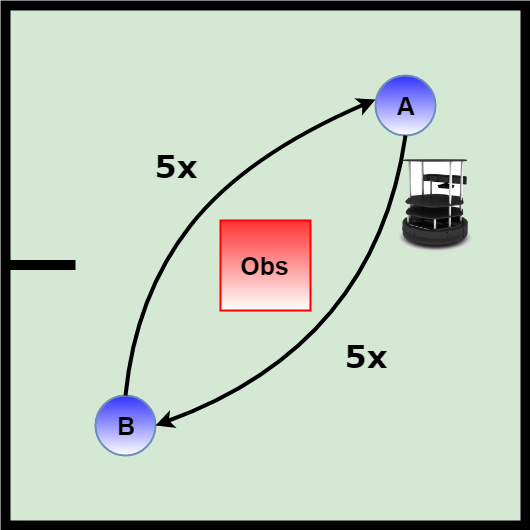
\includegraphics [width=0.5 \textwidth]{imgs/chapter5/exp.png}}
\caption[Demonstration of the course of test]{Demonstration of the course of test, the robot will go back and forth from position A to position B 5 times while  trying to avoid the obstacle in the middle}
\label{fig:exp}
\end{figure}

If the obstacle detection system fails then the robot should collide with said object, if it succeeds the robot should go around the object leaving in between a relatively safe distance. 
%The test was made using the \ac{FMCW} radar, the 2D \ac{LiDAR}, and the fusion of both for different types of objects. 
The  navigation data was recorded in a rosbag file in order to be analyzed later.

The list of objects used as obstacles are displayed in Fig. \ref{fig:obstacles}.
\begin{figure}[h!]
  \centering
  \begin{subfigure}[b]{0.3\linewidth}
    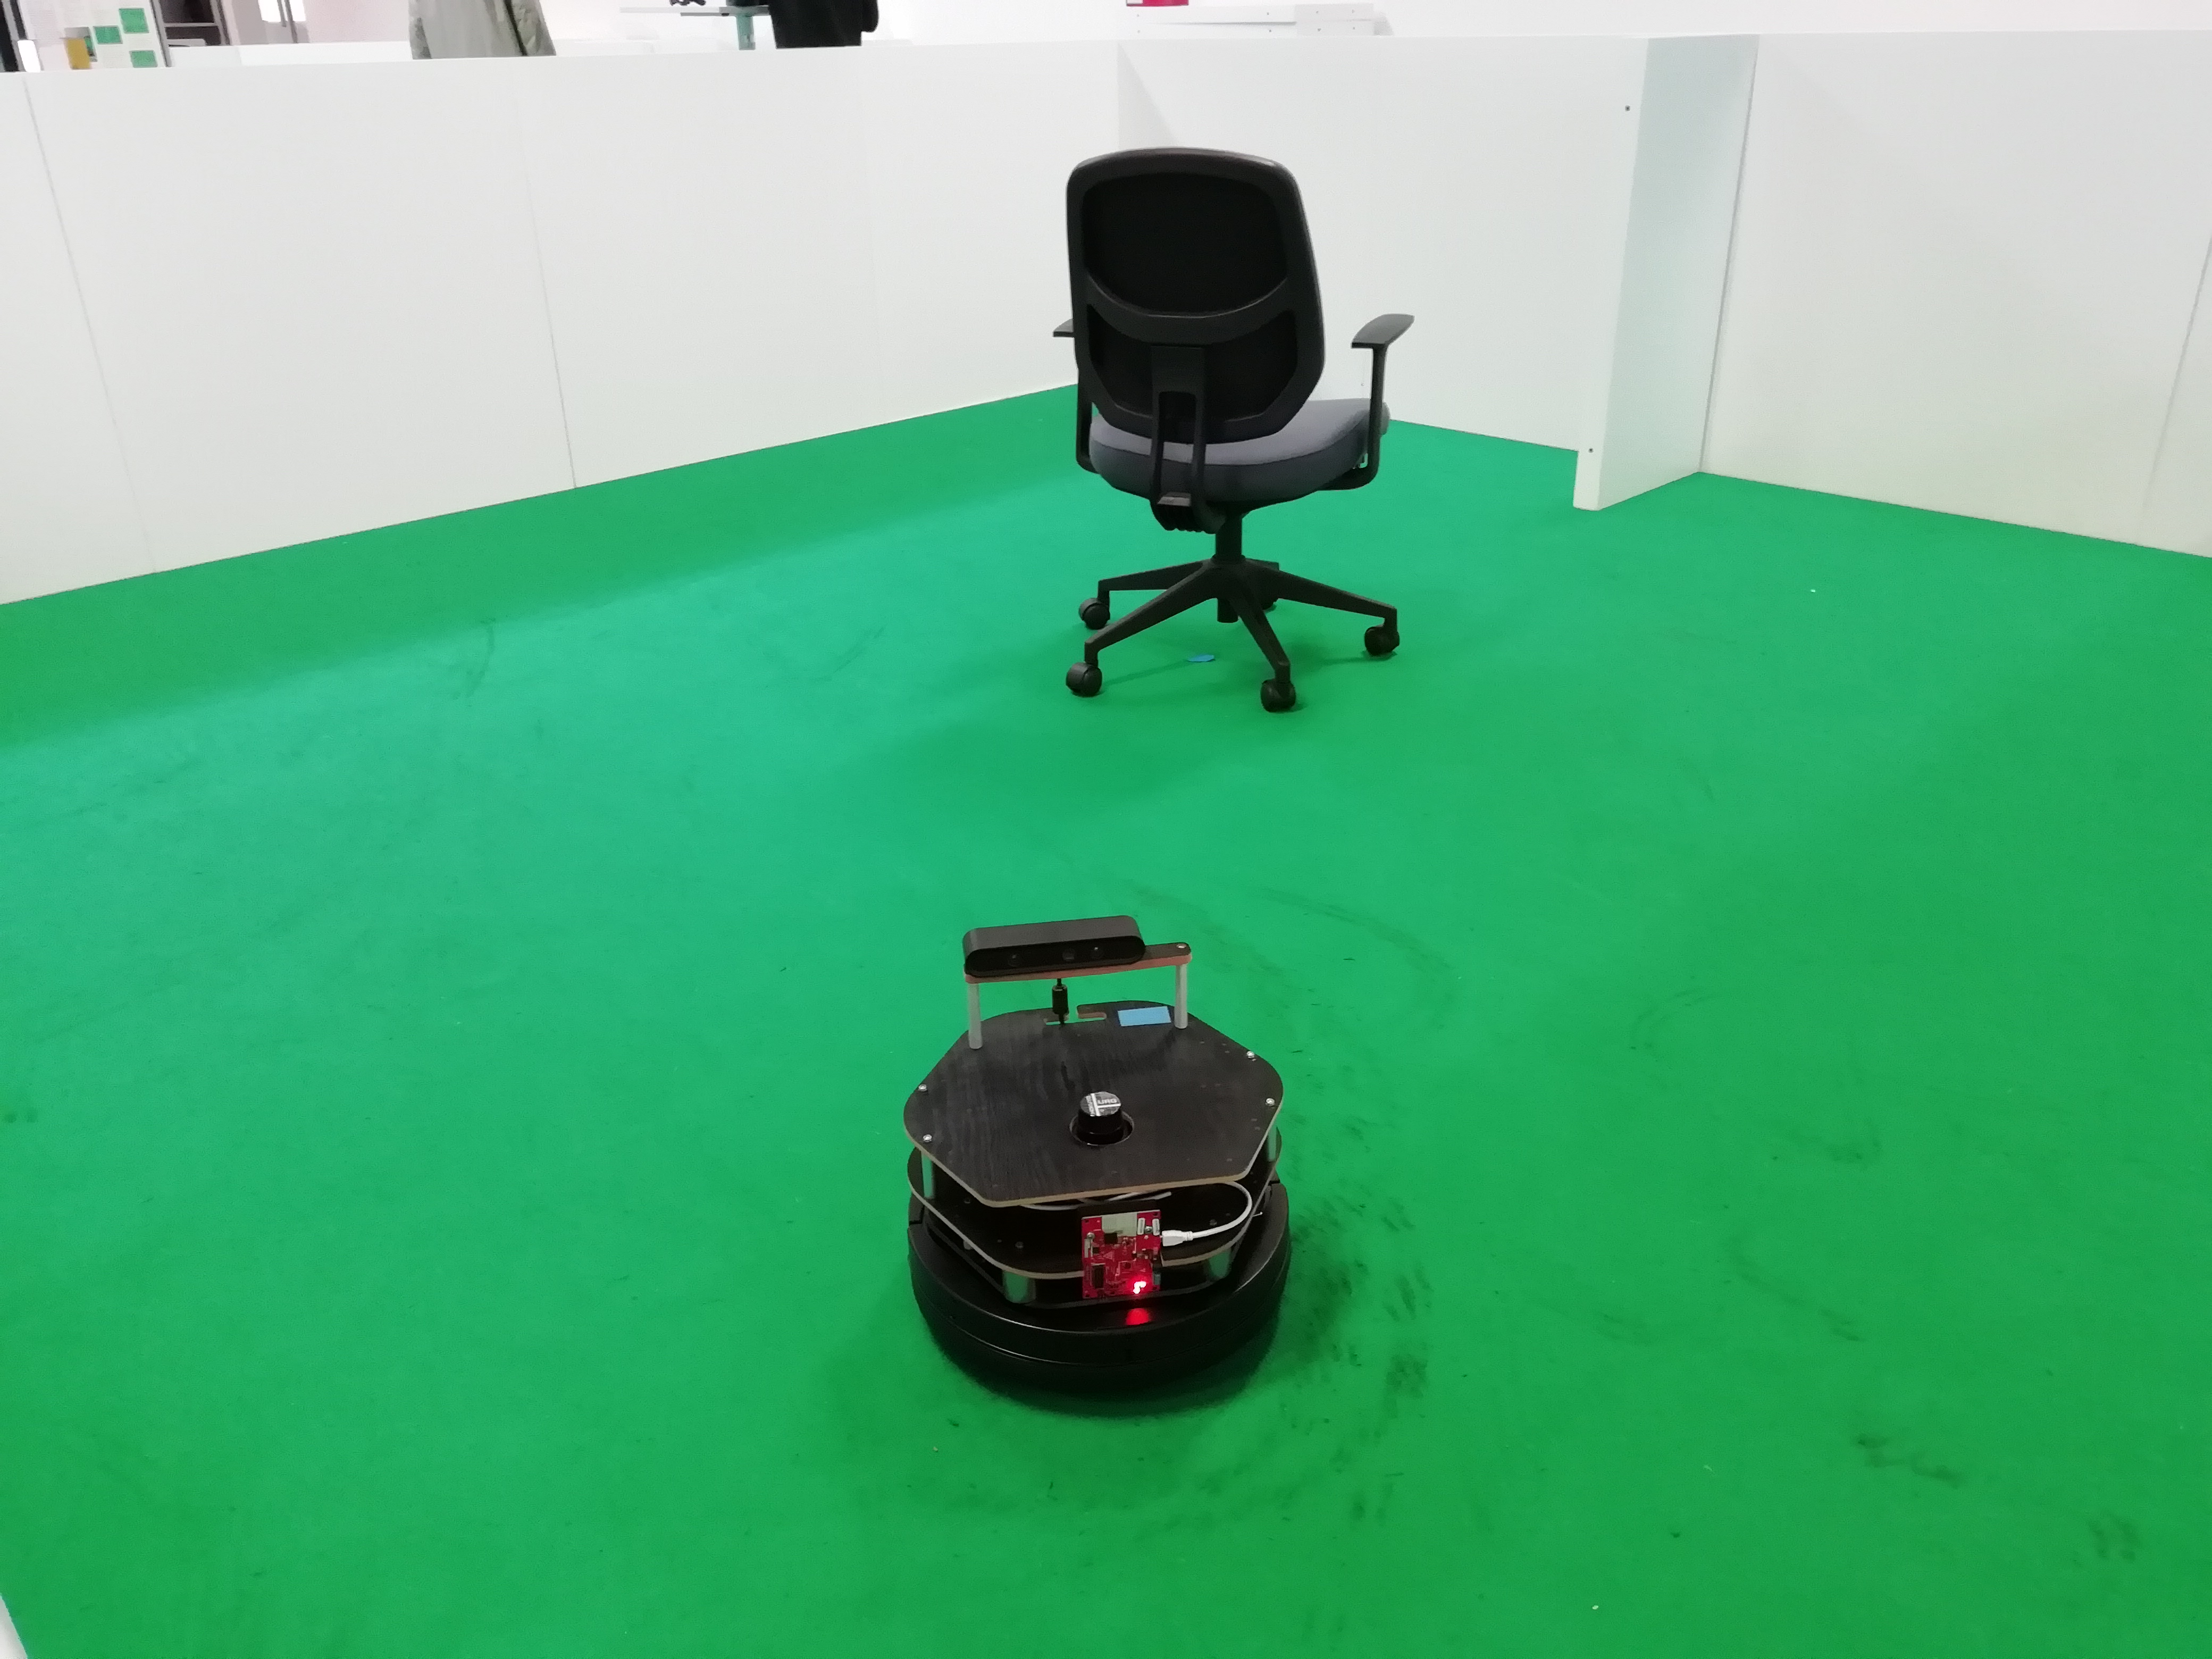
\includegraphics[width=\linewidth]{imgs/chapter5/wchair.jpg}
     \caption{Office chair}
     \label{fig::wchair}
  \end{subfigure}
  \begin{subfigure}[b]{0.3\linewidth}
    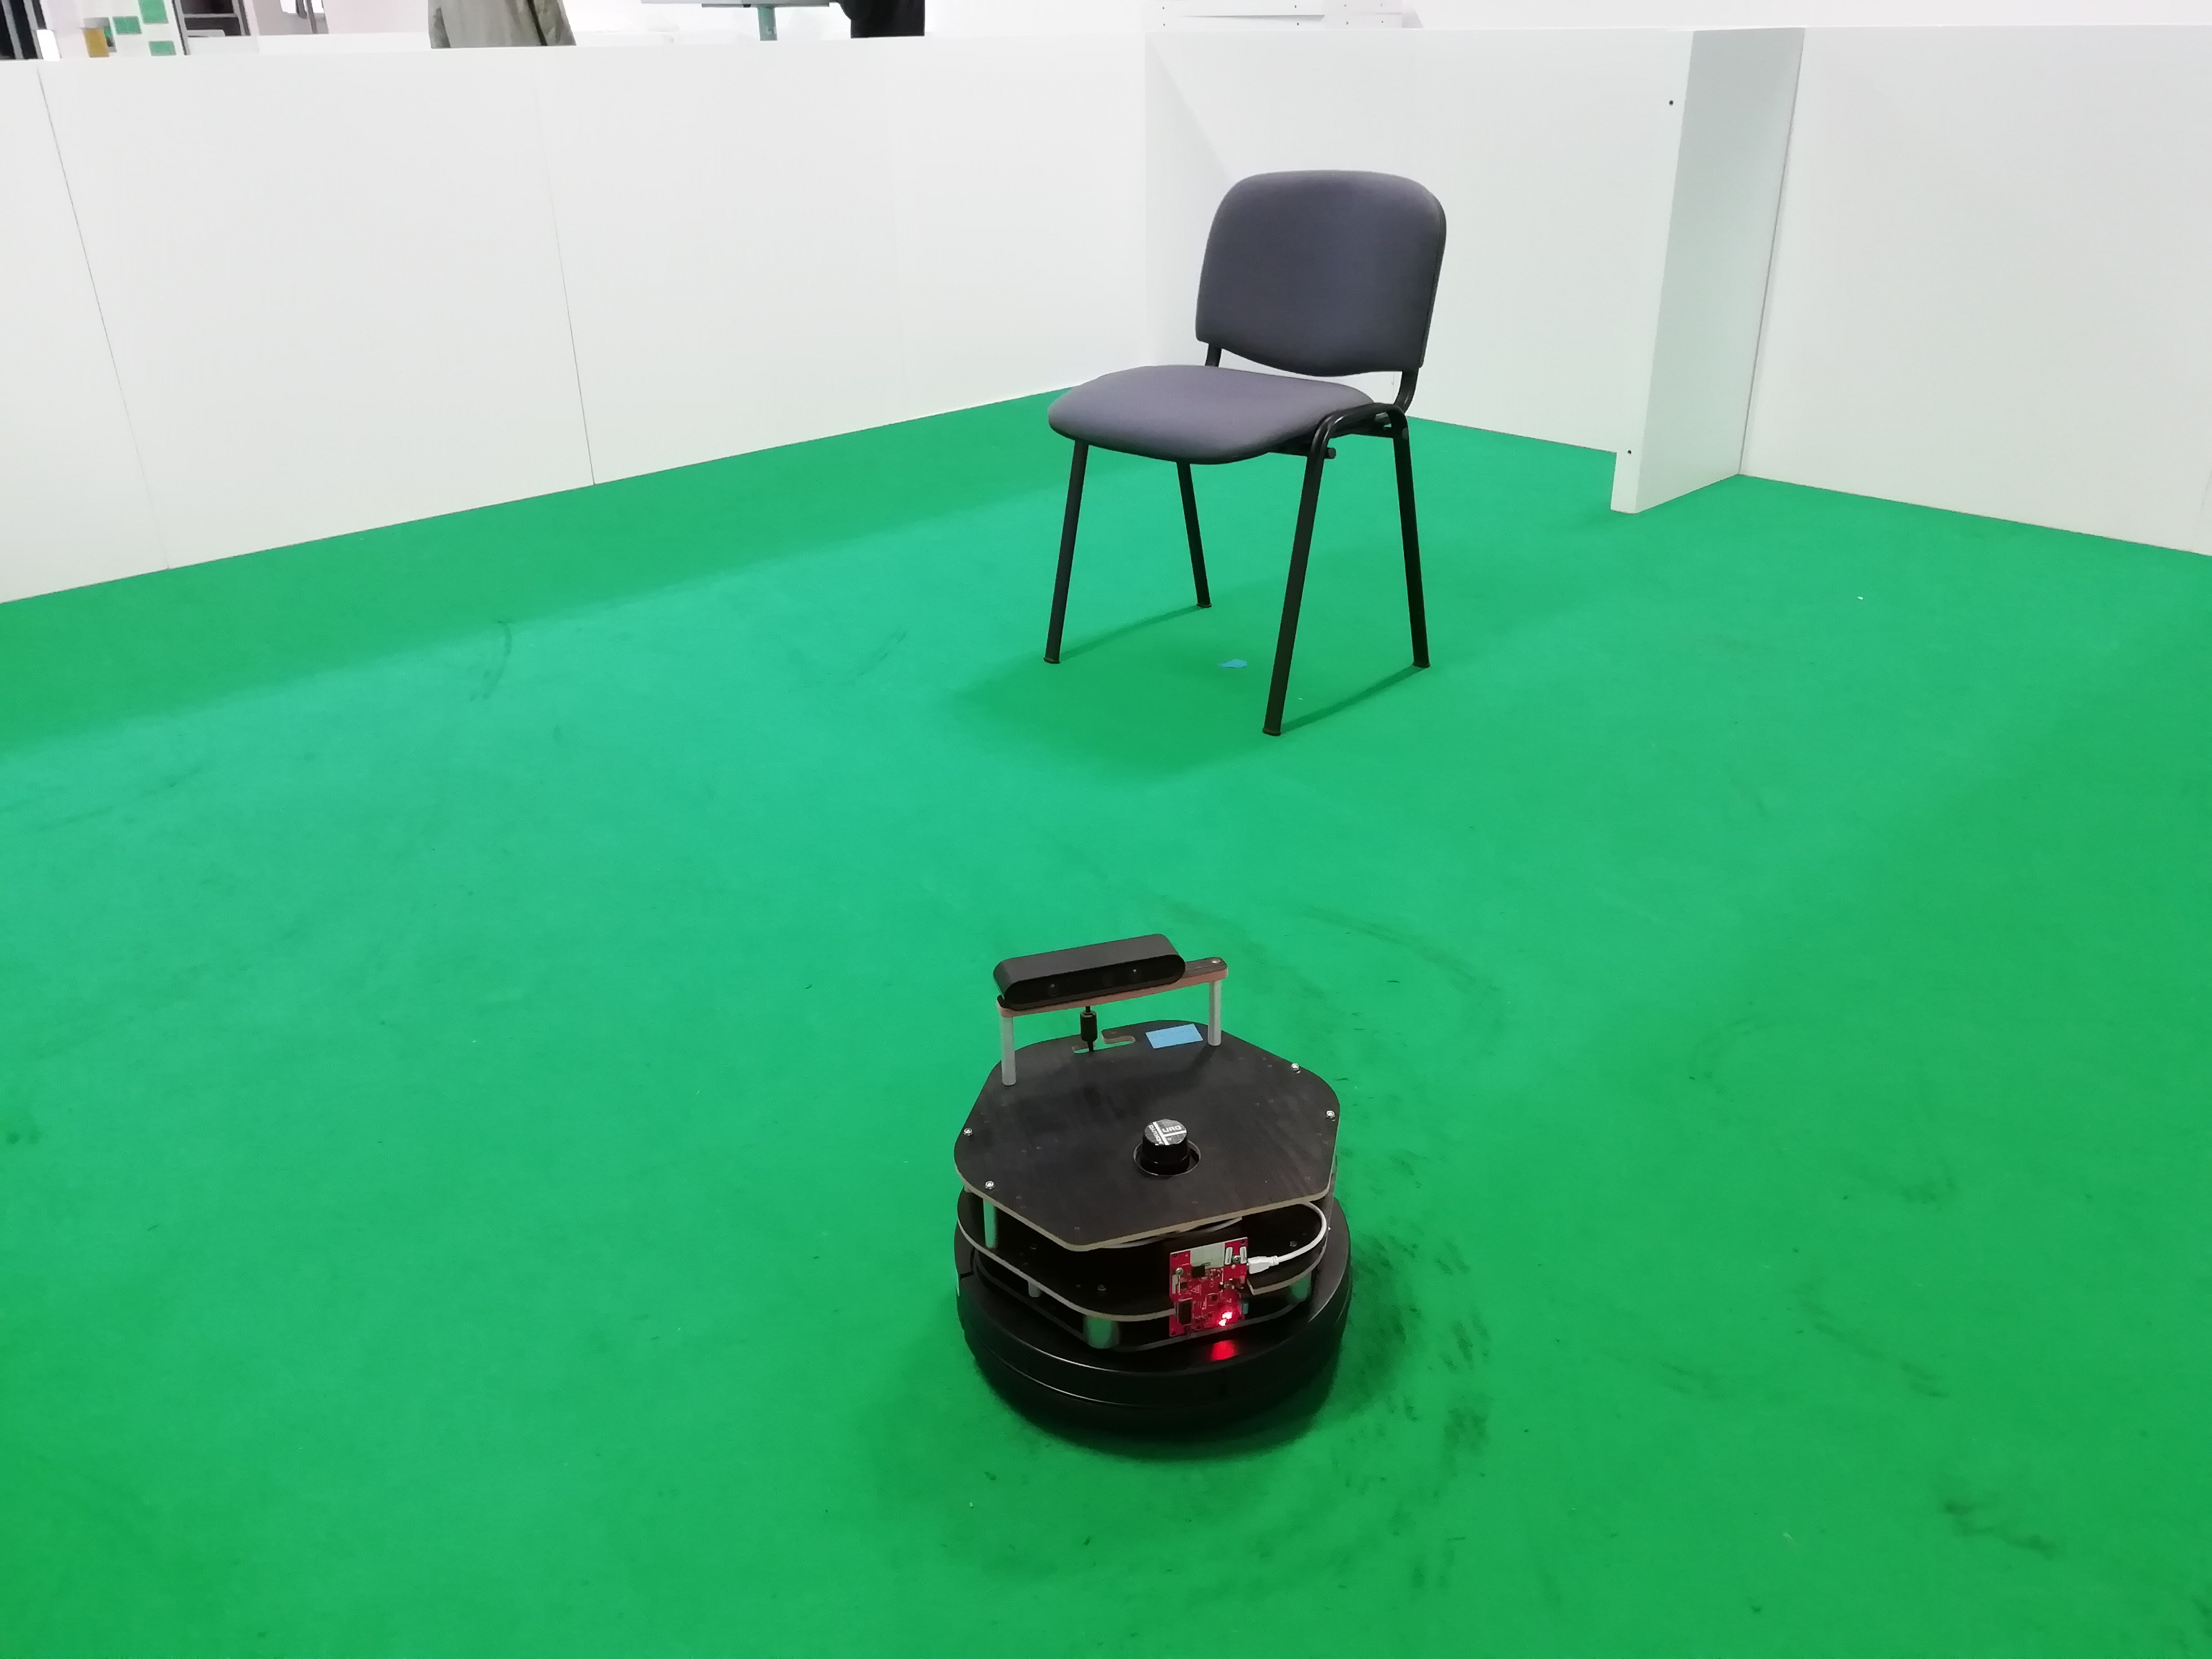
\includegraphics[width=\linewidth]{imgs/chapter5/nchair.jpg}
    \caption{Four legged chair}
    \label{fig::nchair}
  \end{subfigure}
  \begin{subfigure}[b]{0.3\linewidth}
    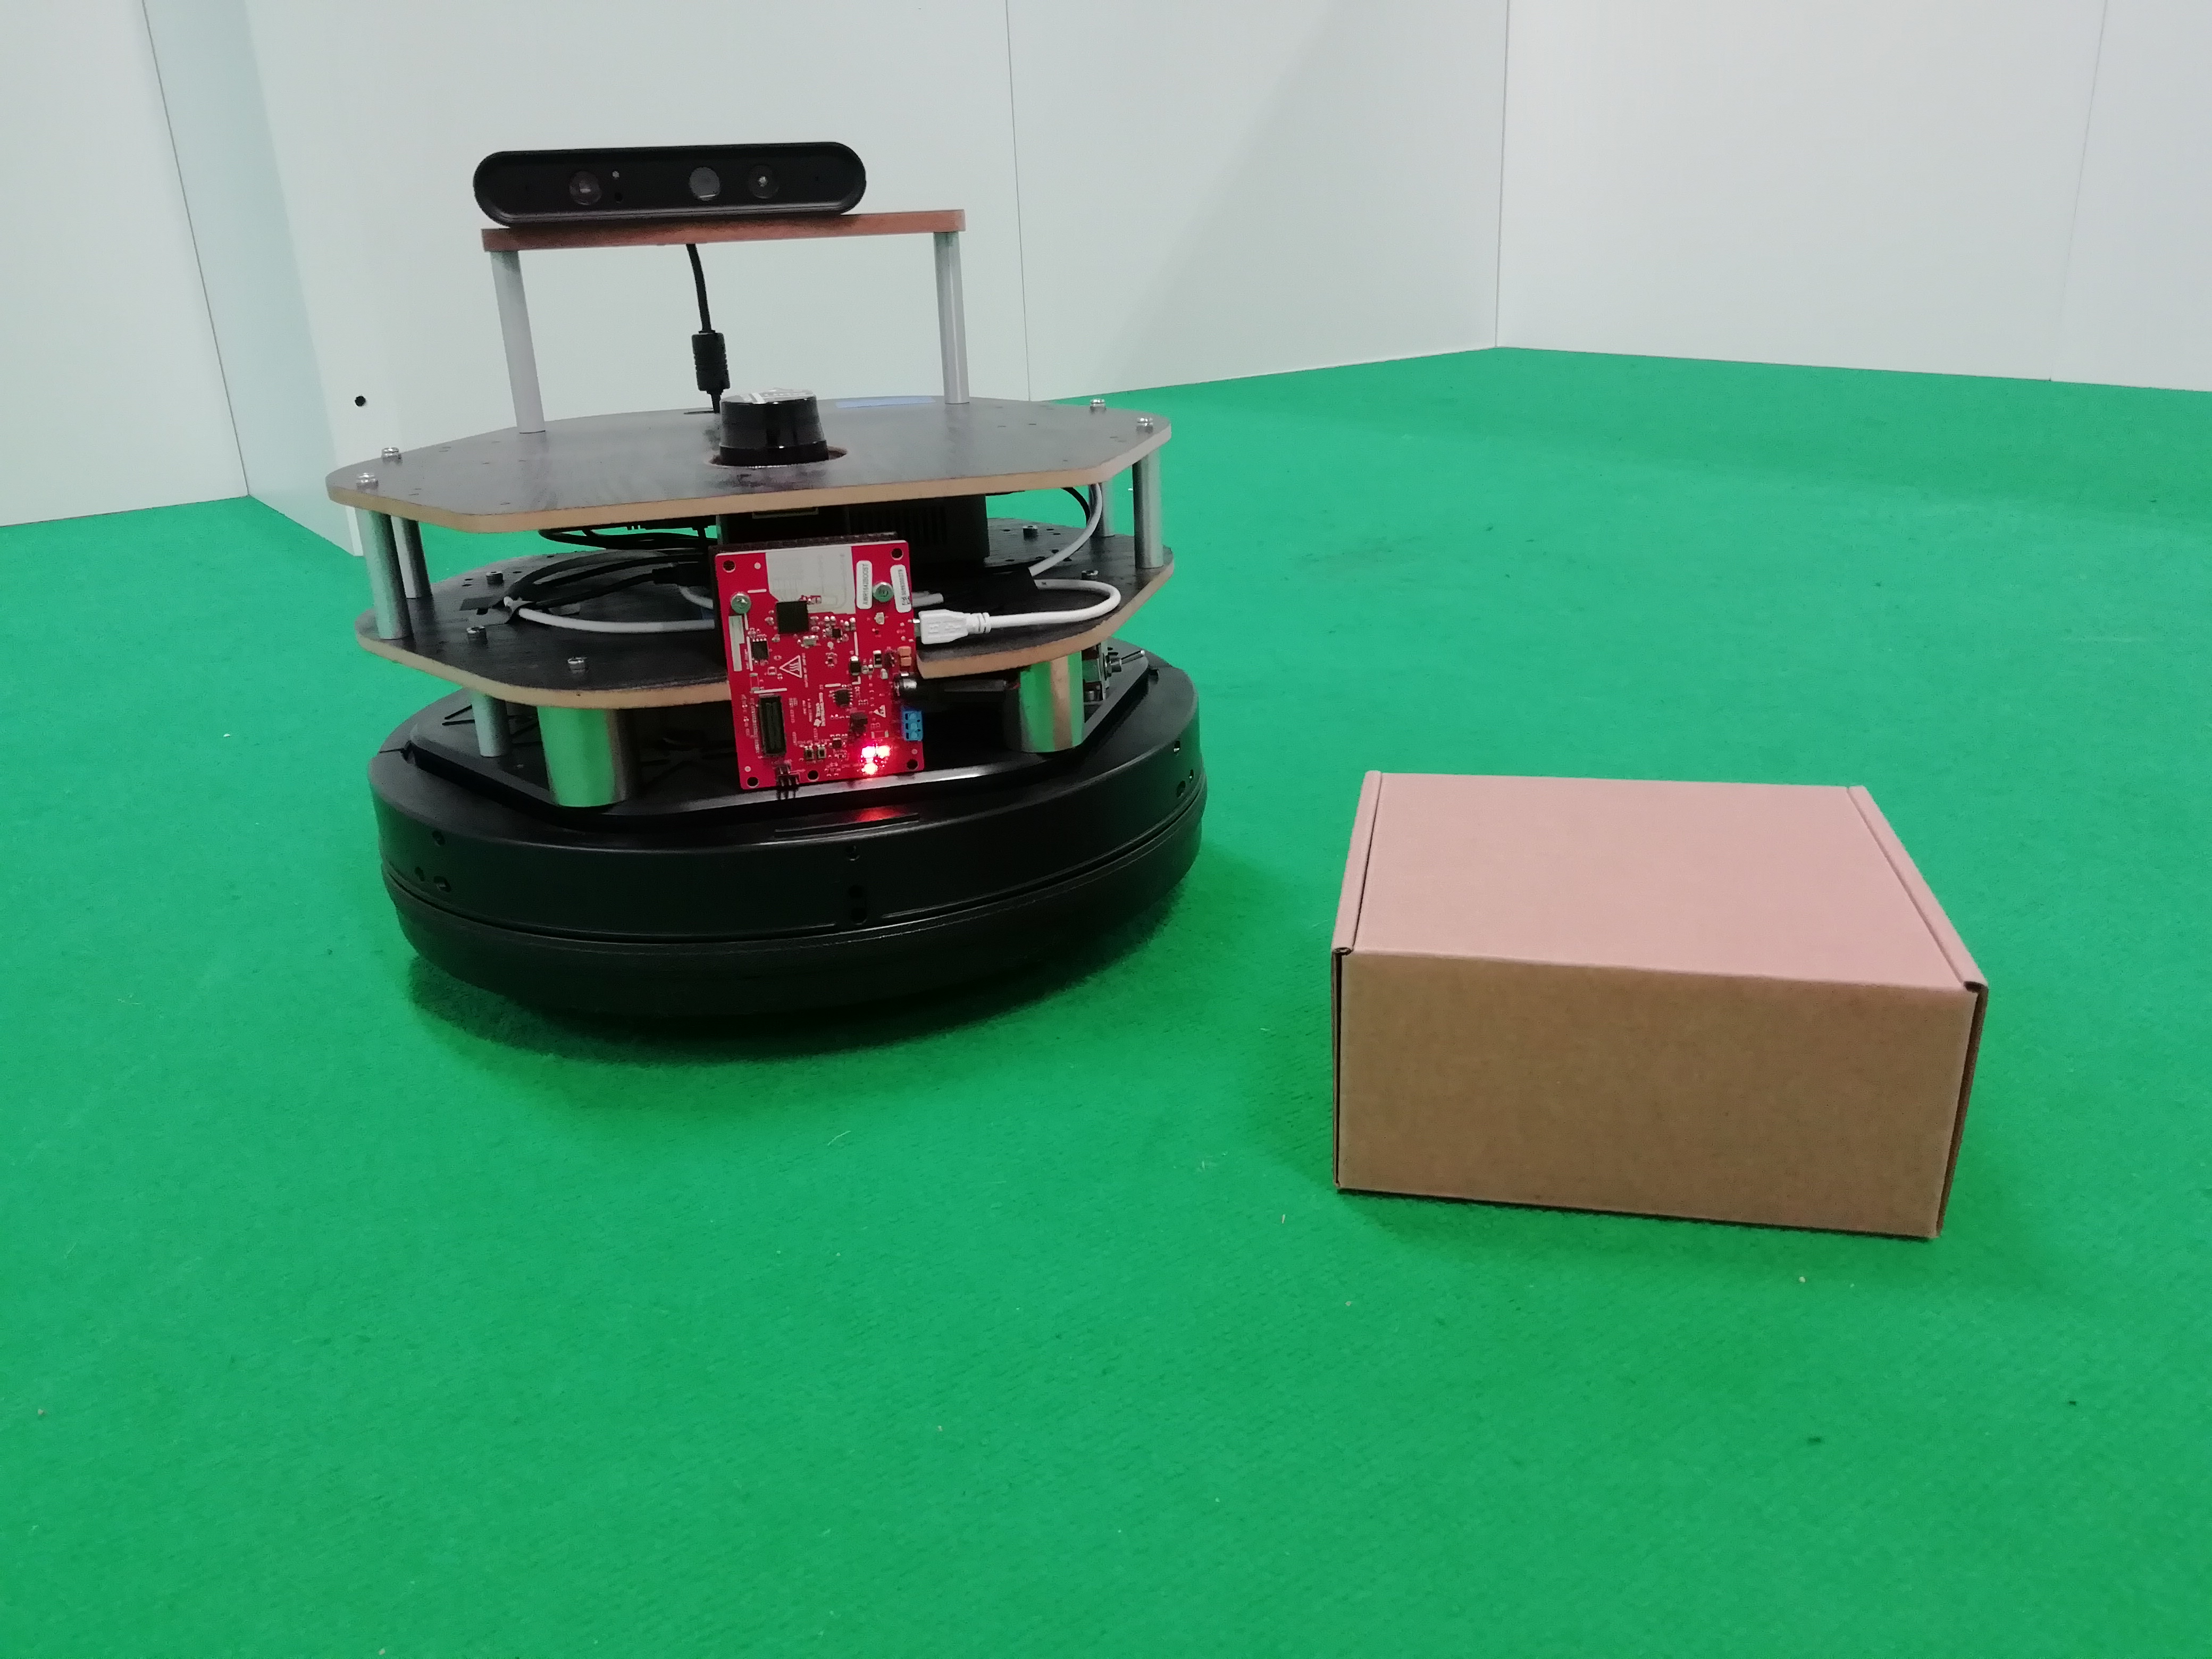
\includegraphics[width=\linewidth]{imgs/chapter5/box.jpg}
    \caption{Low height box}
    \label{fig::box}
  \end{subfigure}
  \begin{subfigure}[b]{0.3\linewidth}
    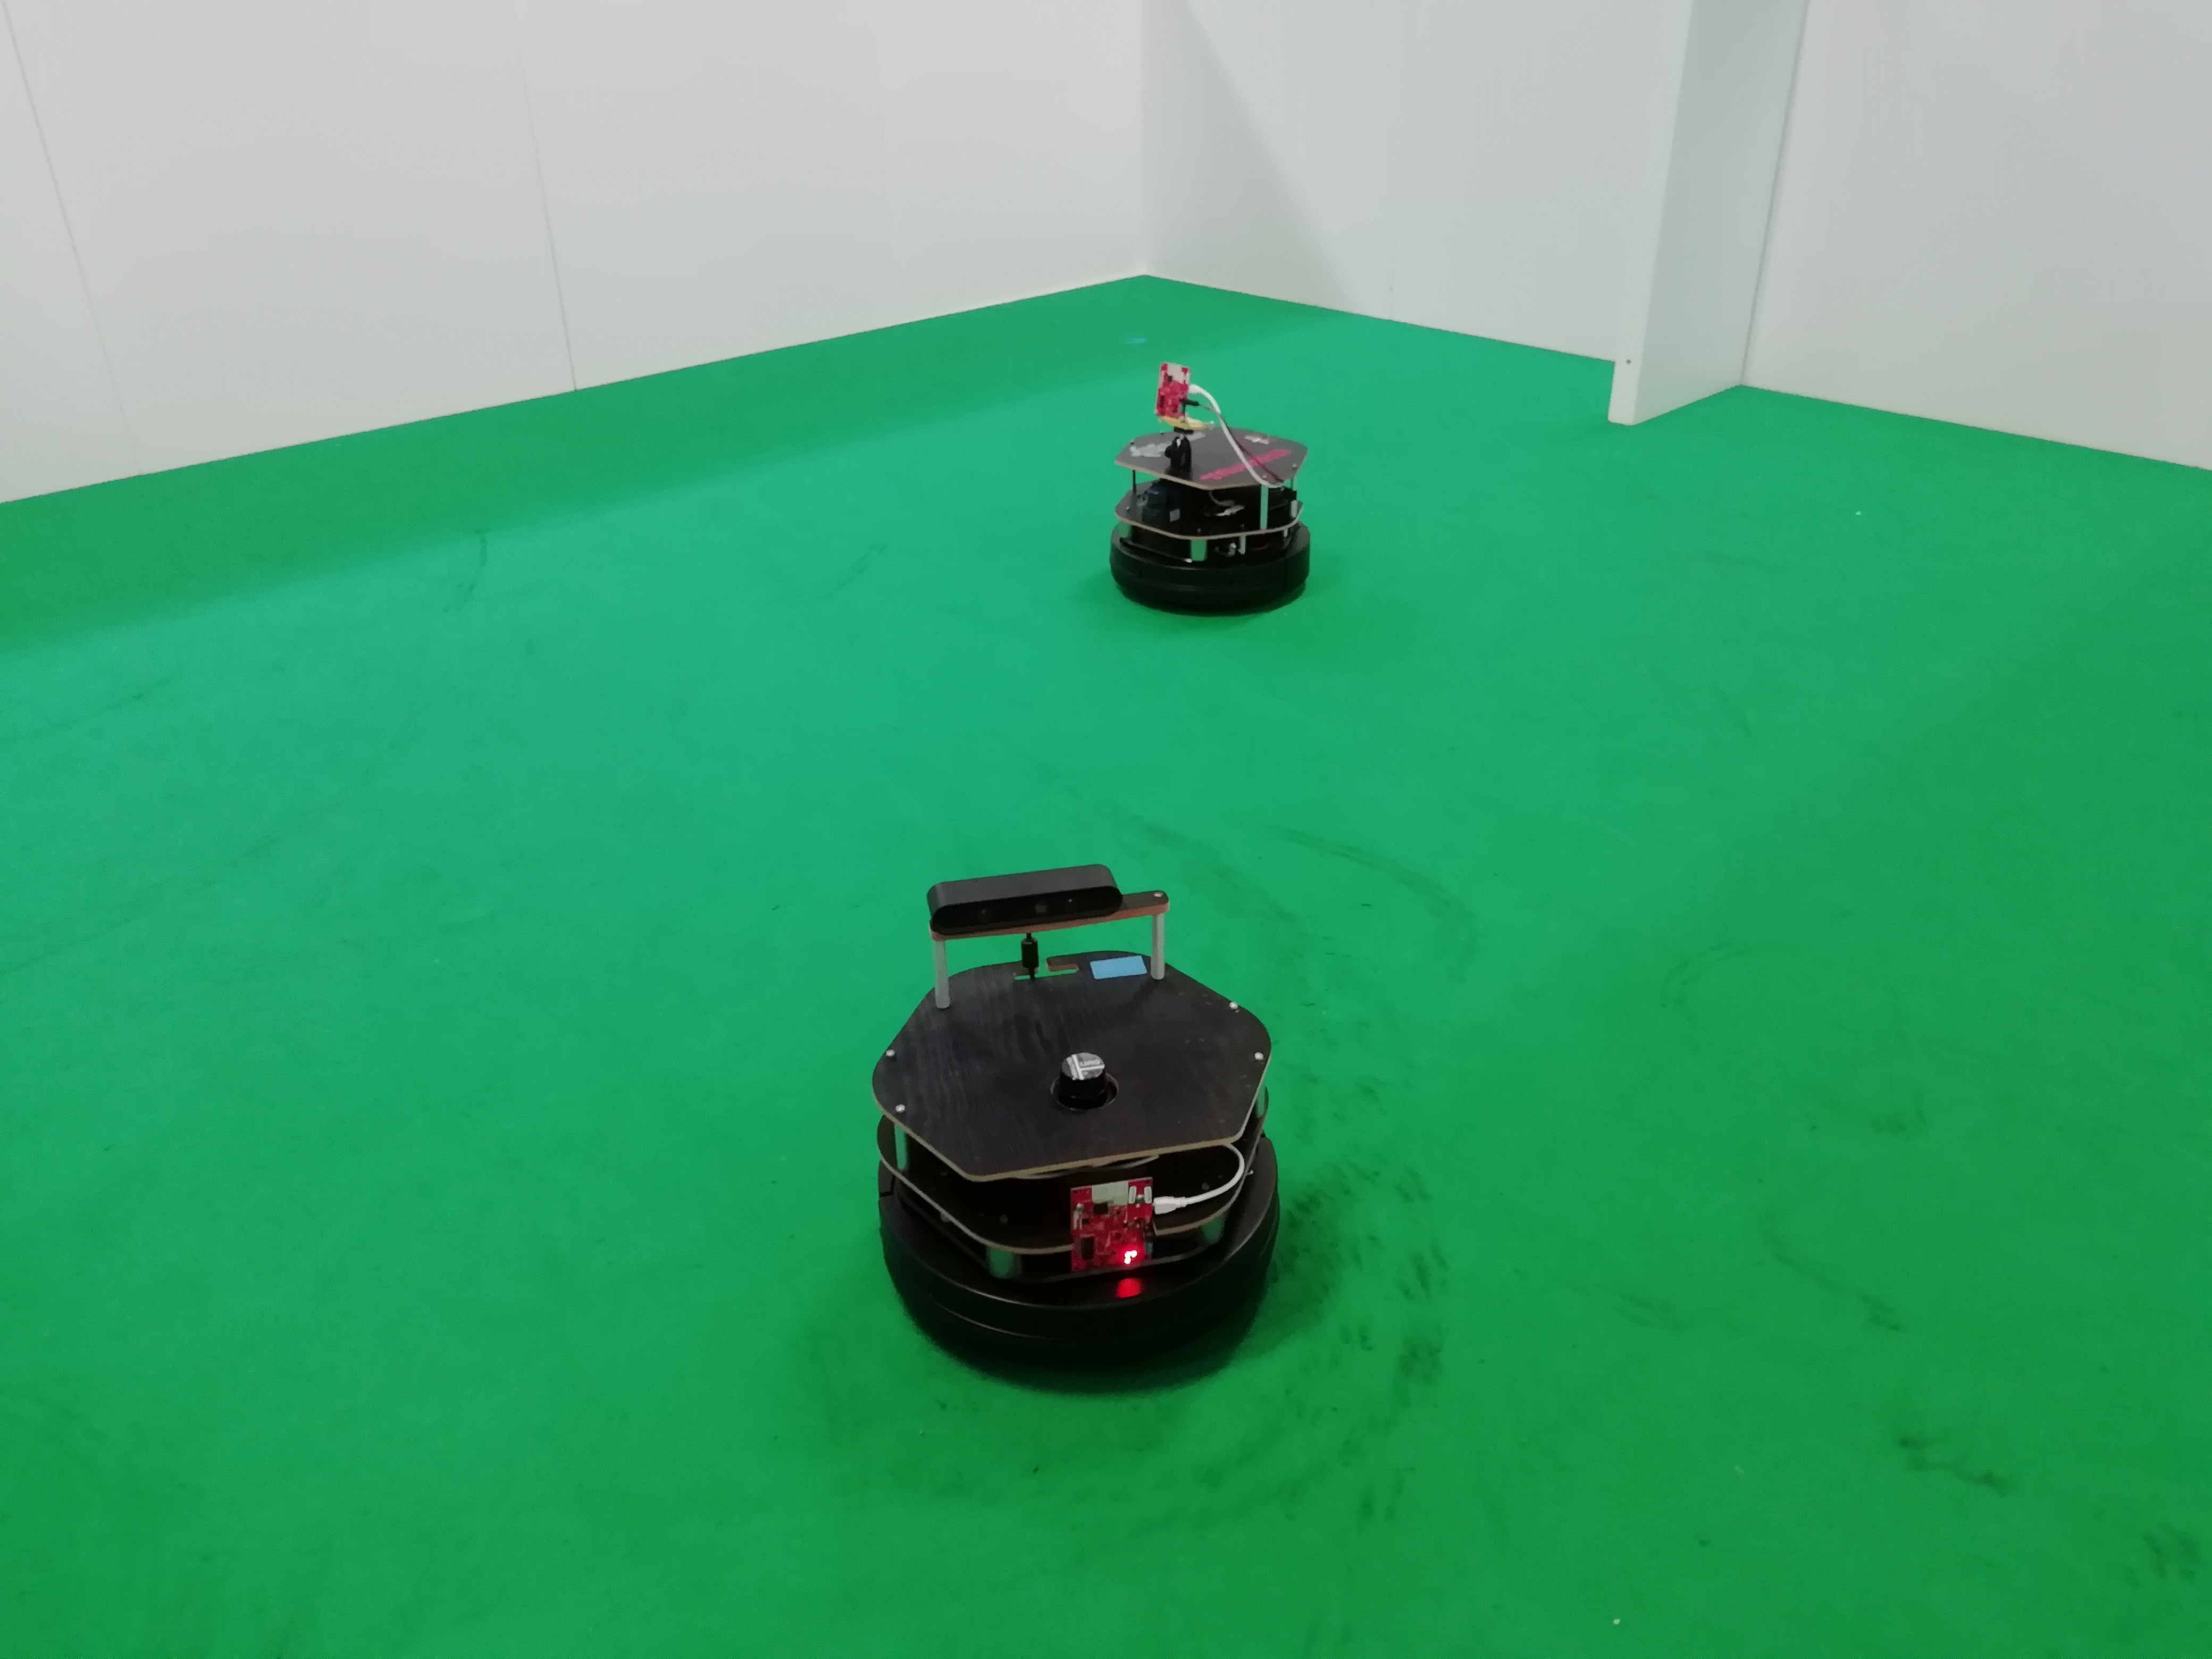
\includegraphics[width=\linewidth]{imgs/chapter5/robot.jpg}
    \caption{Another turtlebot}
    \label{fig::robot}
  \end{subfigure}
  \begin{subfigure}[b]{0.3\linewidth}
    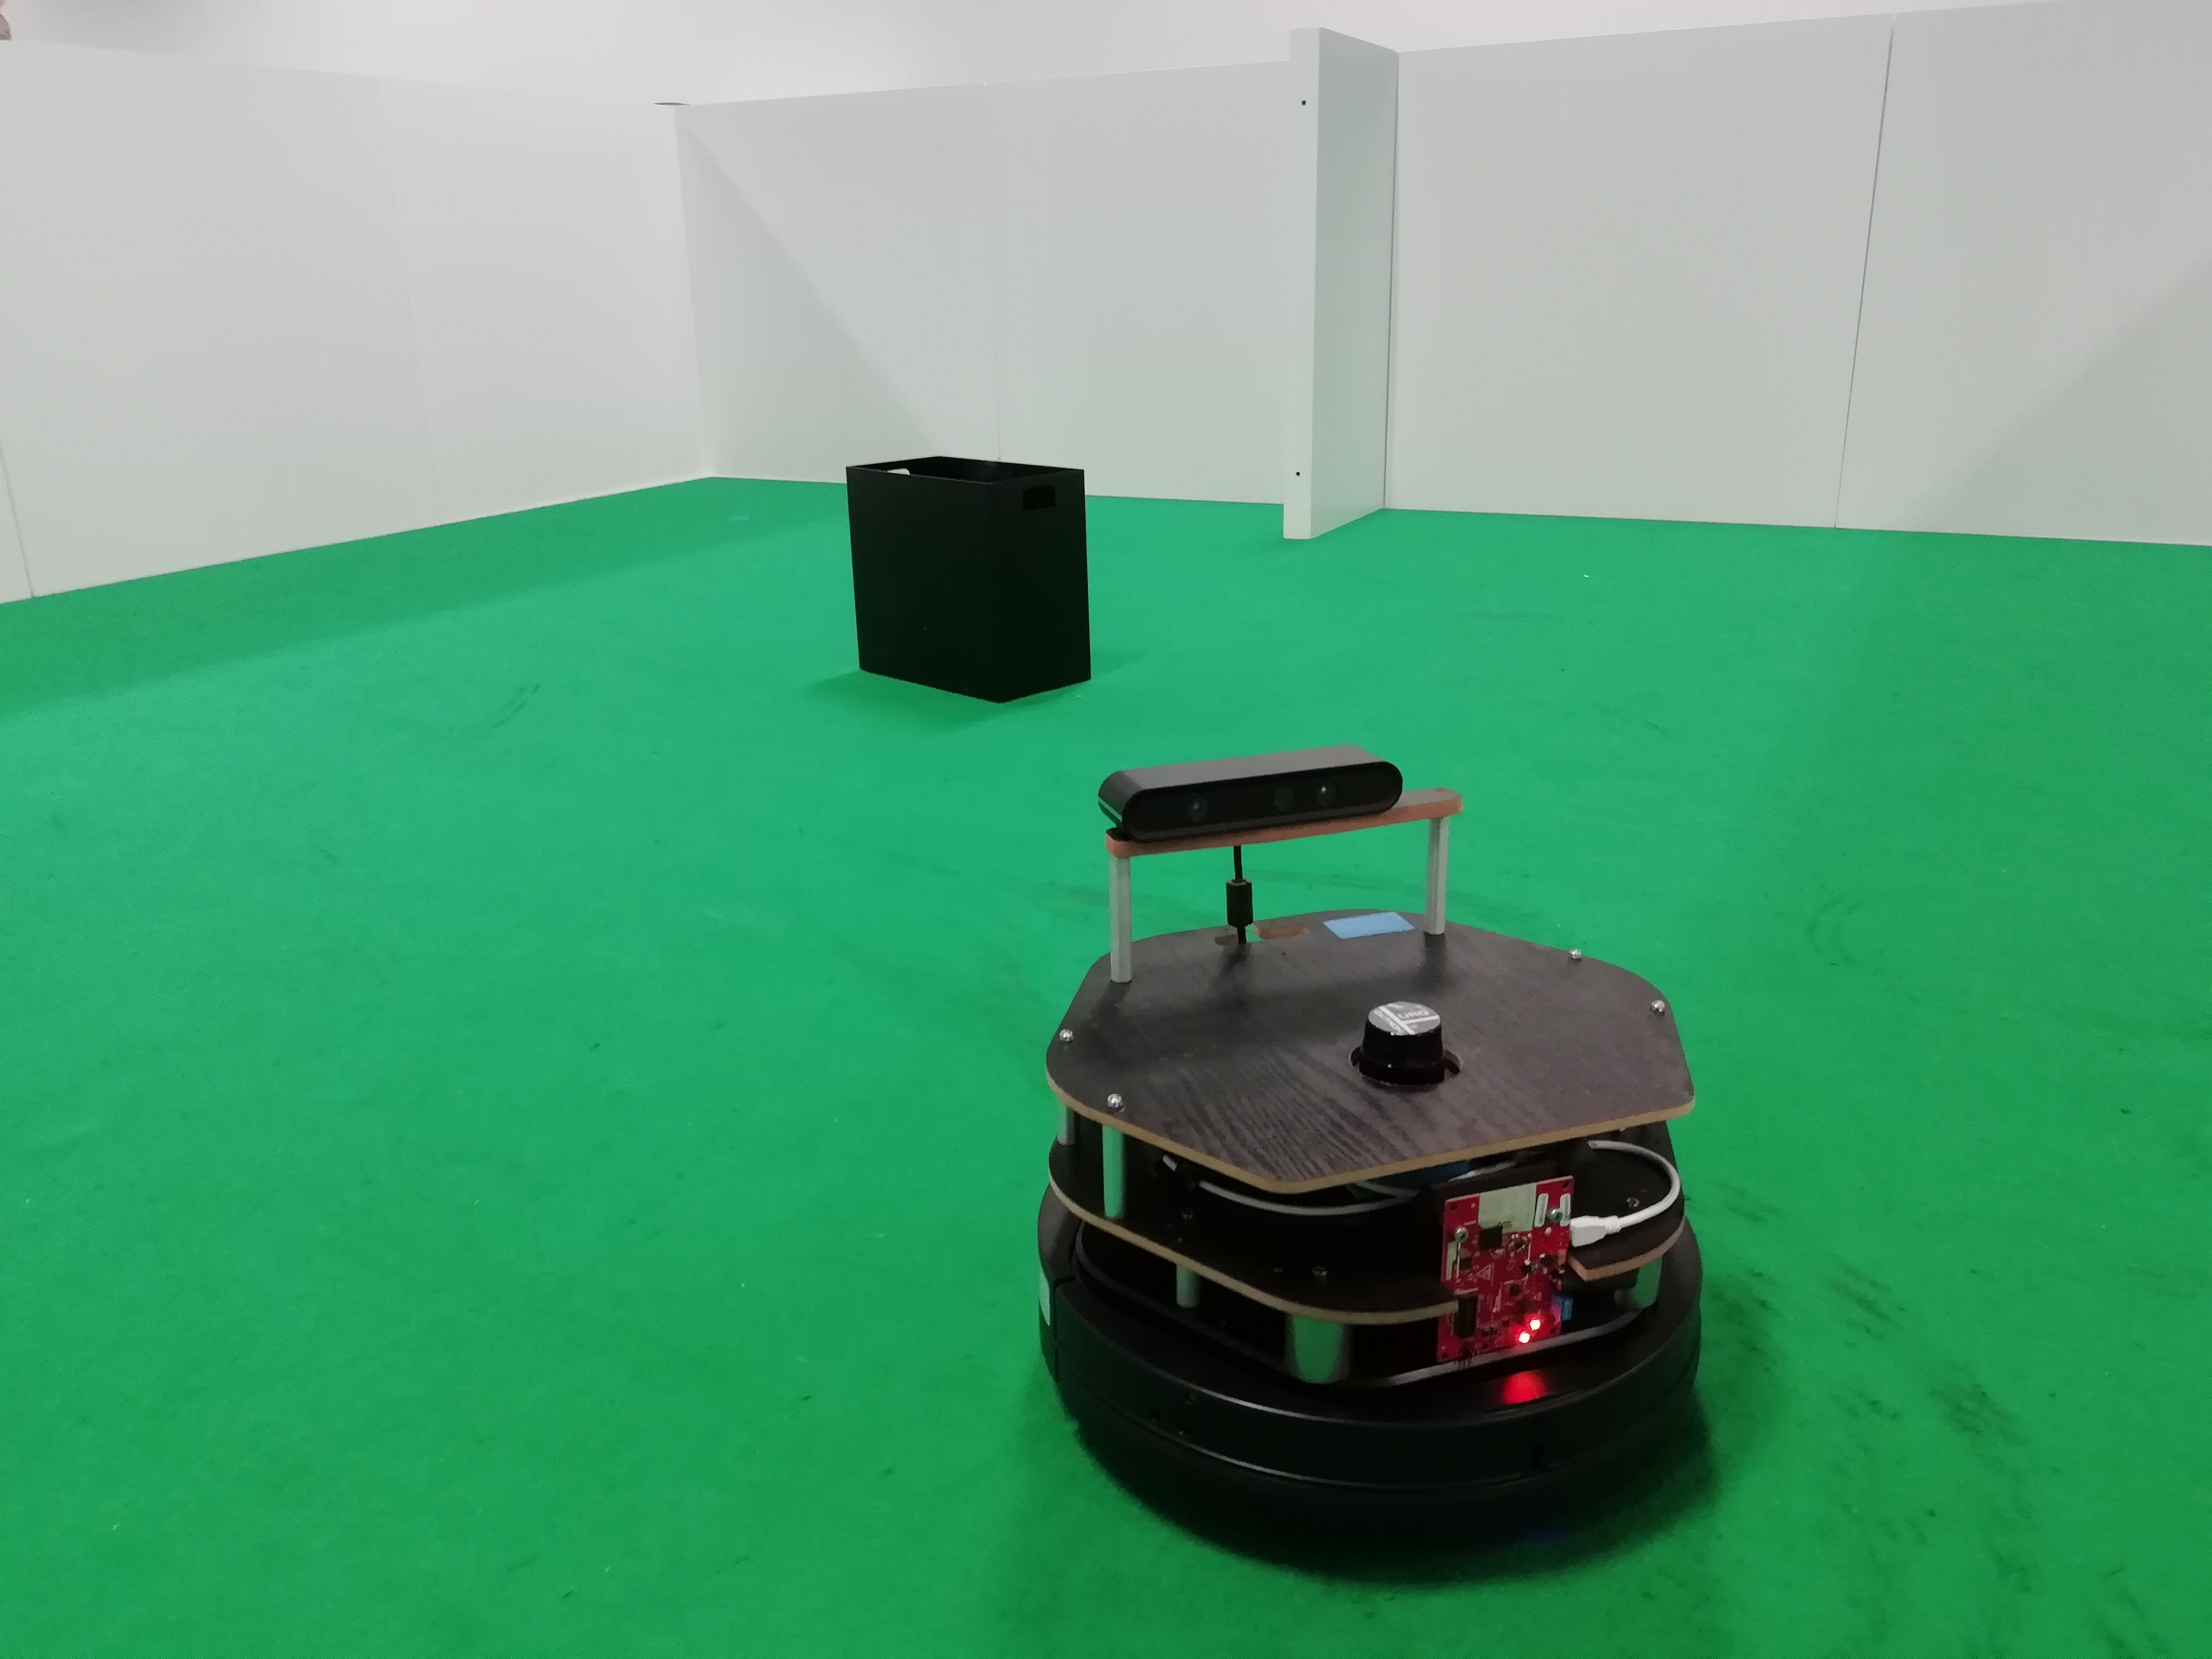
\includegraphics[width=\linewidth]{imgs/chapter5/garbage.jpg}
    \caption{Garbage Bin}
    \label{fig::garbage}
  \end{subfigure}
  \begin{subfigure}[b]{0.3\linewidth}
    \includegraphics[width=\linewidth]{imgs/chapter5/glass.jpg}
    \caption{Acrylic tube}
    \label{fig::garbage}
  \end{subfigure}
  \caption{Different obstacles used for the controlled test}
  \label{fig:obstacles}
\end{figure}

\subsection{Results}
In this section we show the results of how the robot performed in avoiding the previous obstacles using different type of sensor sources (\ac{FMCW} radar, the 2D \ac{LiDAR} and both).

\subsubsection{Office Chair}







\subsubsection*{\ac{LiDAR}}
In the \ac{LiDAR}'s case  the robot completely disregarded the chair going in a straight line and pushing it until it was away from the experimental setup has shown in Figure \ref{fig:wchairLF}.

\begin{figure}[h!]
  \centering
  \begin{subfigure}[b]{0.49\linewidth}
    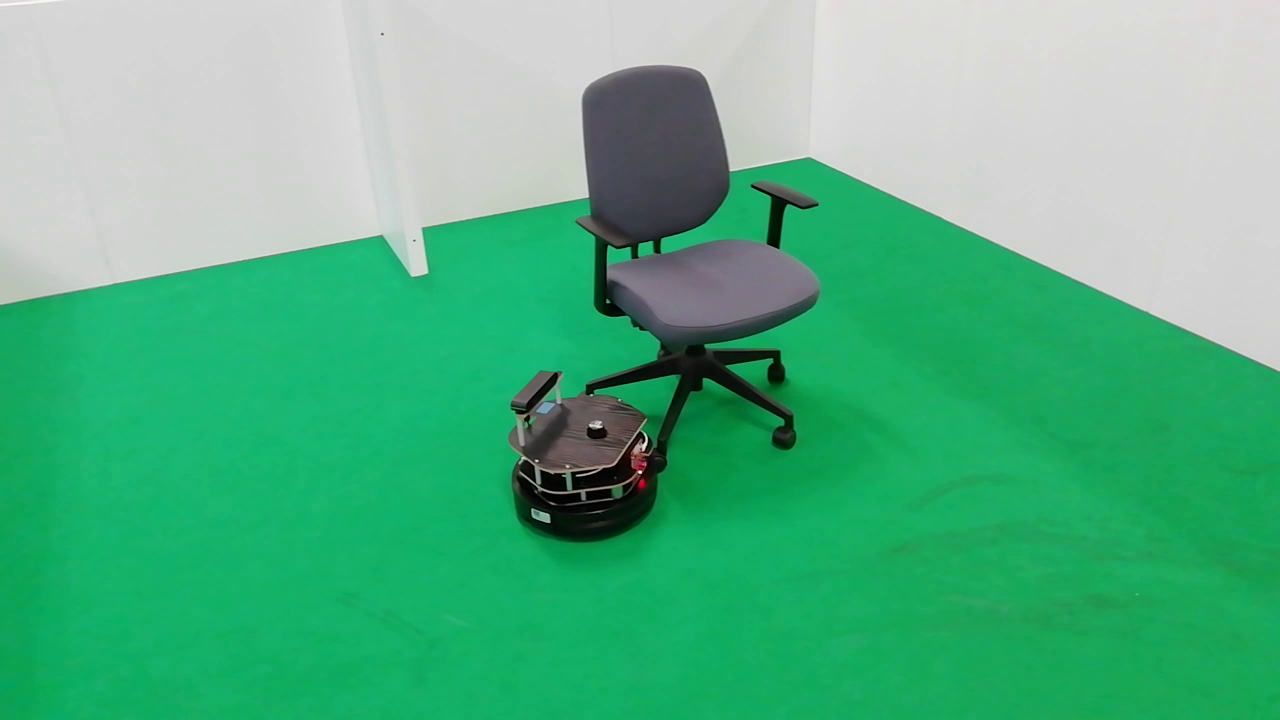
\includegraphics[width=\linewidth]{imgs/chapter5/wchairLF.png}
     \caption{Robot collision with office chair number 1}
     \label{fig::wchair}
  \end{subfigure}
  \begin{subfigure}[b]{0.49\linewidth}
    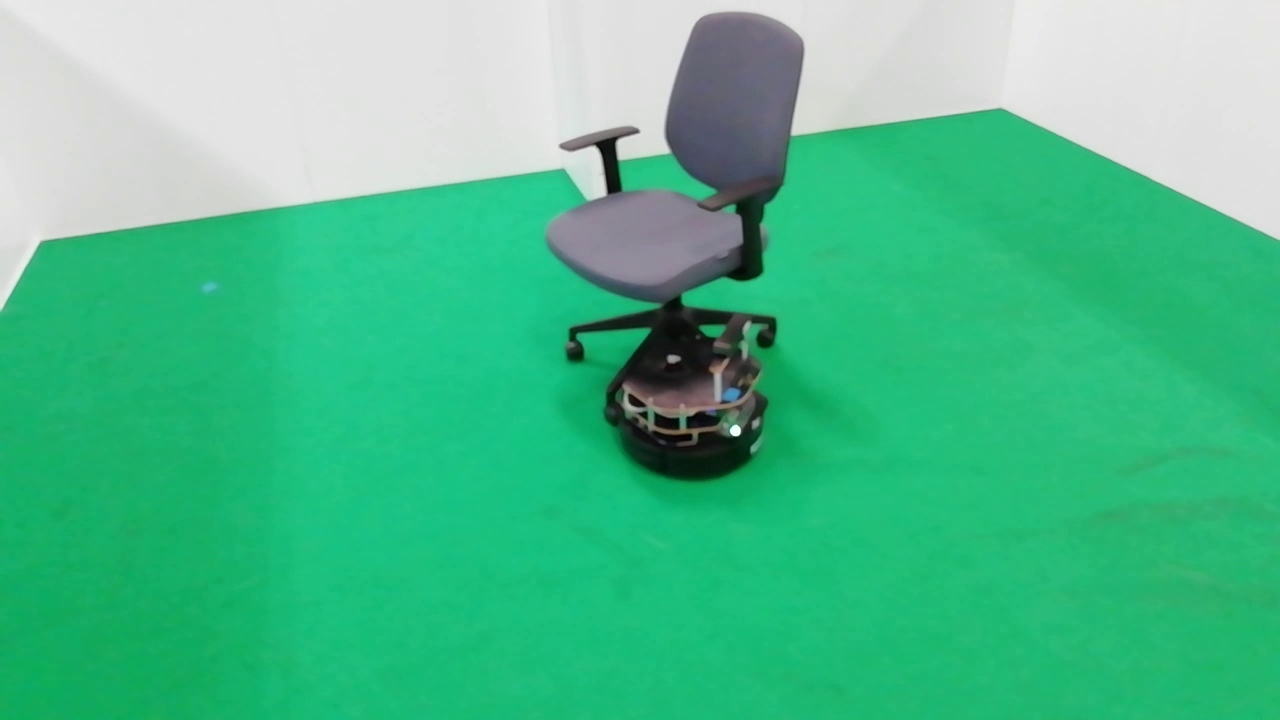
\includegraphics[width=\linewidth]{imgs/chapter5/wchairLF2.png}
    \caption{Robot collision with office chair number 2}
    \label{fig::nchair}
  \end{subfigure}
  \caption{Robot colliding multiple times with office chair}
  \label{fig:wchairLF}
\end{figure}






This was due to the 2D \ac{LiDAR} only detecting the leg of the chair and not the wheels. This means that the robot only perceived a single point as being occupied and not the full area of the chair. Although the inflation layer  might correct this error in some cases, since the detection is so late the robot still was unable to avoid it.

\subsubsection*{\ac{FMCW} \ac{radar}}
However with the \ac{FMCW} radar the chair is detected almost immediately, this makes the global planner and motion controller to be able to adjust in a very comfortable way and with it the robot is able to avoid collision. Figure \ref{fig:wchairRS} shows some instances of the first experiment. Although the detected space that the chair is occupying has some mismatch, the early detection makes up for it. However since the radar has small field of view (120 degrees) the robot might not detect the obstacle when it is passing by it which in this case lead to it scraping by the chair one time.

\begin{figure}[h!]
  \centering
  \begin{subfigure}[b]{0.49\linewidth}
    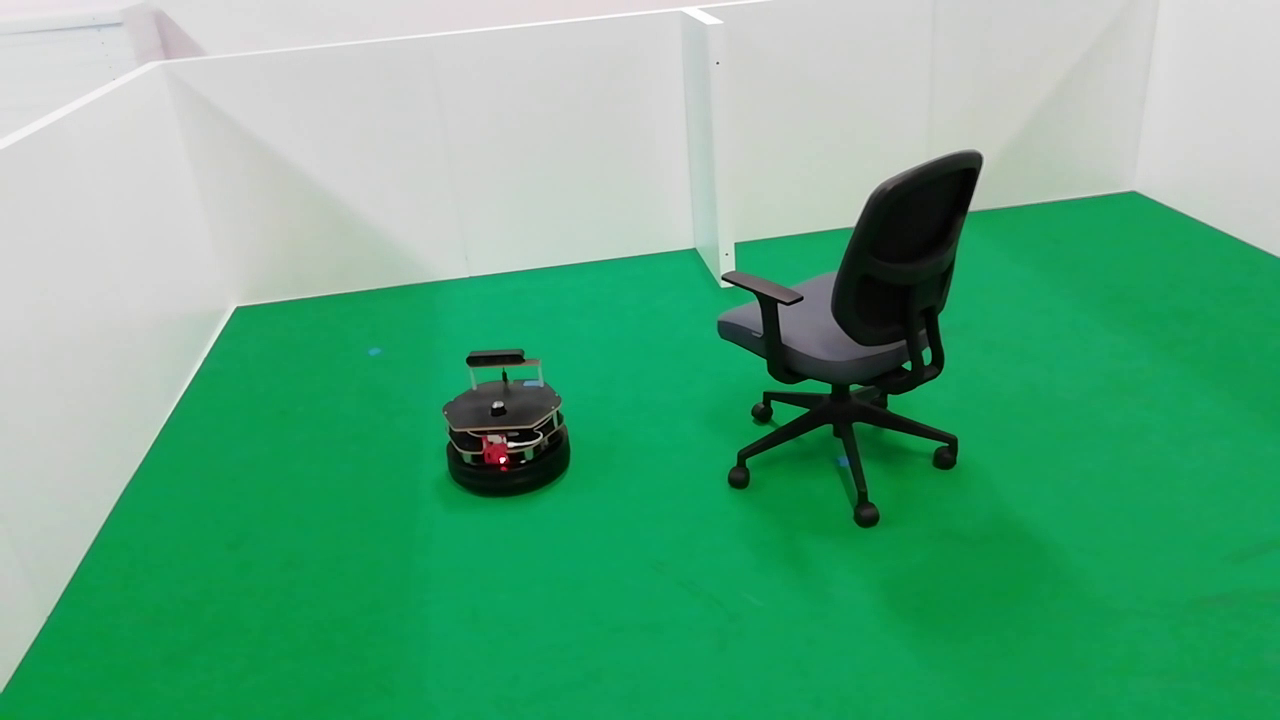
\includegraphics[width=\linewidth]{imgs/chapter5/wchairRS.png}
     \caption{Robot avoiding office chair number 1}
     \label{fig::wchair}
  \end{subfigure}
  \begin{subfigure}[b]{0.49\linewidth}
    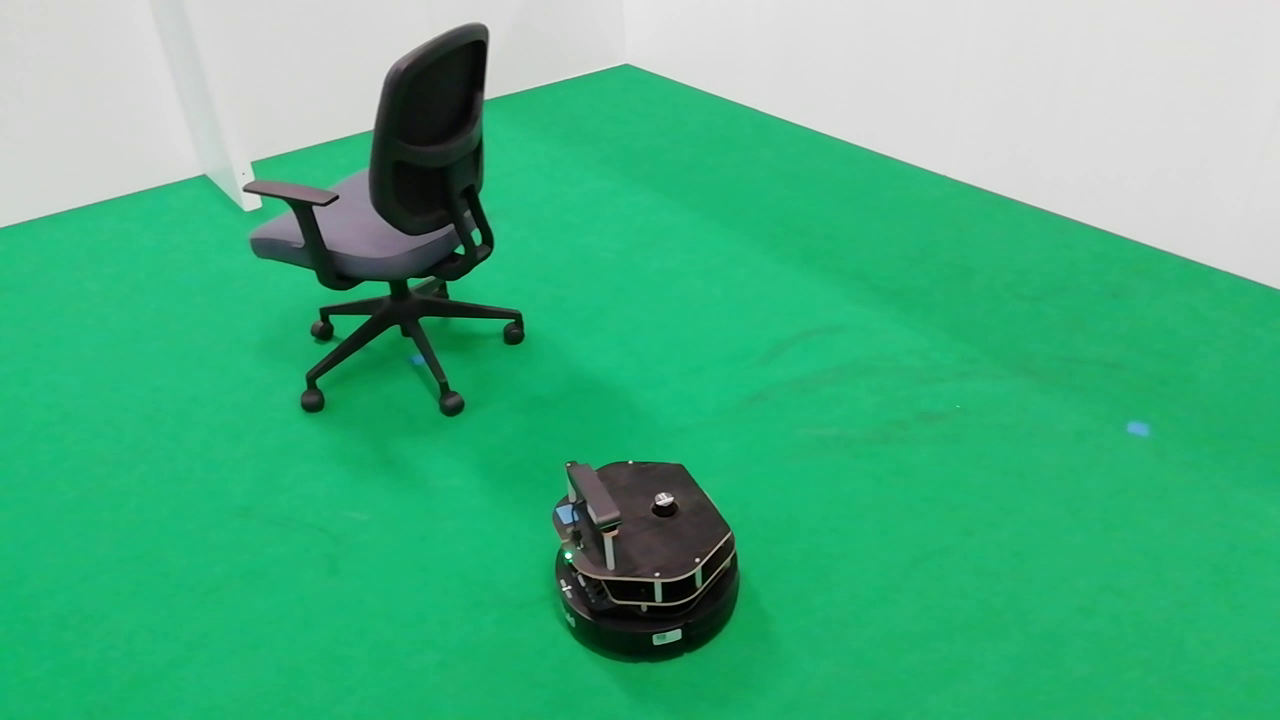
\includegraphics[width=\linewidth]{imgs/chapter5/wchairRS2.png}
    \caption{Robot avoiding office chair number 2}
    \label{fig::nchair}
  \end{subfigure}
  \caption{Robot avoiding with office chair}
  \label{fig:wchairRS}
\end{figure}

\subsubsection*{Robot Trajectory}
Figure \ref{fig:traj1} shows the robot trajectory in the \ac{LiDAR} and the \ac{FMCW} radar case aswell an aproximation of the of the invalid space the  center of the robot can not go through in dimmed red. As we can see the robot flat out ignores the obstacle with \ac{LiDAR} while in the \ac{FMCW} \ac{radar} case it narrowly avoids it at all times.
\begin{figure}[ht!]
\centerline{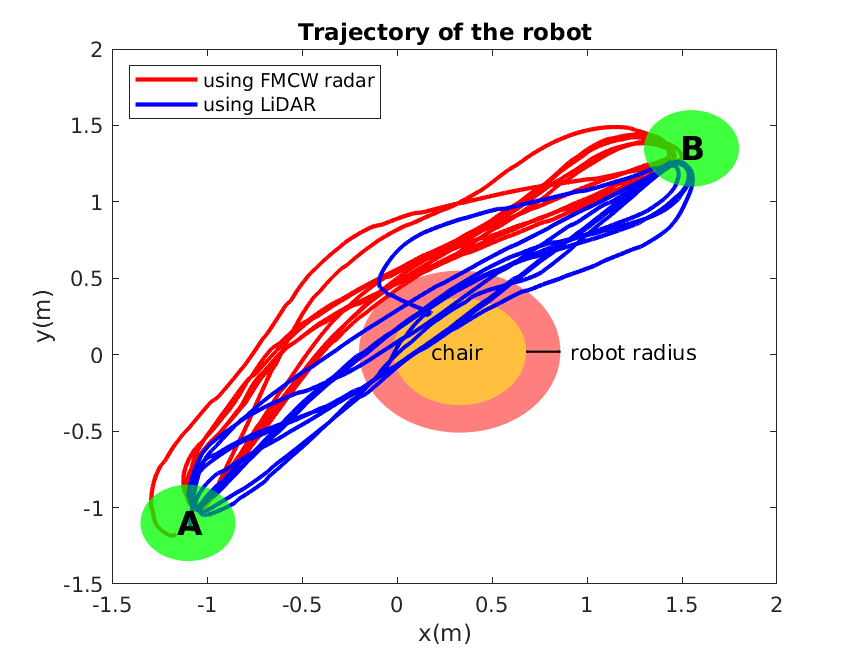
\includegraphics [width=0.7 \textwidth]{imgs/chapter5/traj1.png}}
\caption{Trajectory of the robot for the office chair's case}
\label{fig:traj1}
\end{figure}


\subsubsection{Four Legged Chair}
\subsubsection*{LiDAR}
Using \ac{LiDAR} the robot did not succeed in producing a safe trajectory.

First off it went in a straight line just as the previous case almost hitting  the legs of the chair. However when it got to close to it, it came to a halt and kept oscillating for a long time until it either collided with the leg or scrapping by it. This was again due to the \ac{LiDAR} only detecting this type of obstacle at small distances. This behavior repeated itself throughout the task, leading to the chair being pushed several times. Figure \ref{fig:nchairLF} shows two instances where the robot gets stuck near the chair. This type of behavior is indicative that the robot's motion controller is stuck in local minimum, in other words computing a safe trajectory around the obstacle is countered by its force to follow the goal and path.
\begin{figure}[h!]
  \centering
  \begin{subfigure}[b]{0.49\linewidth}
    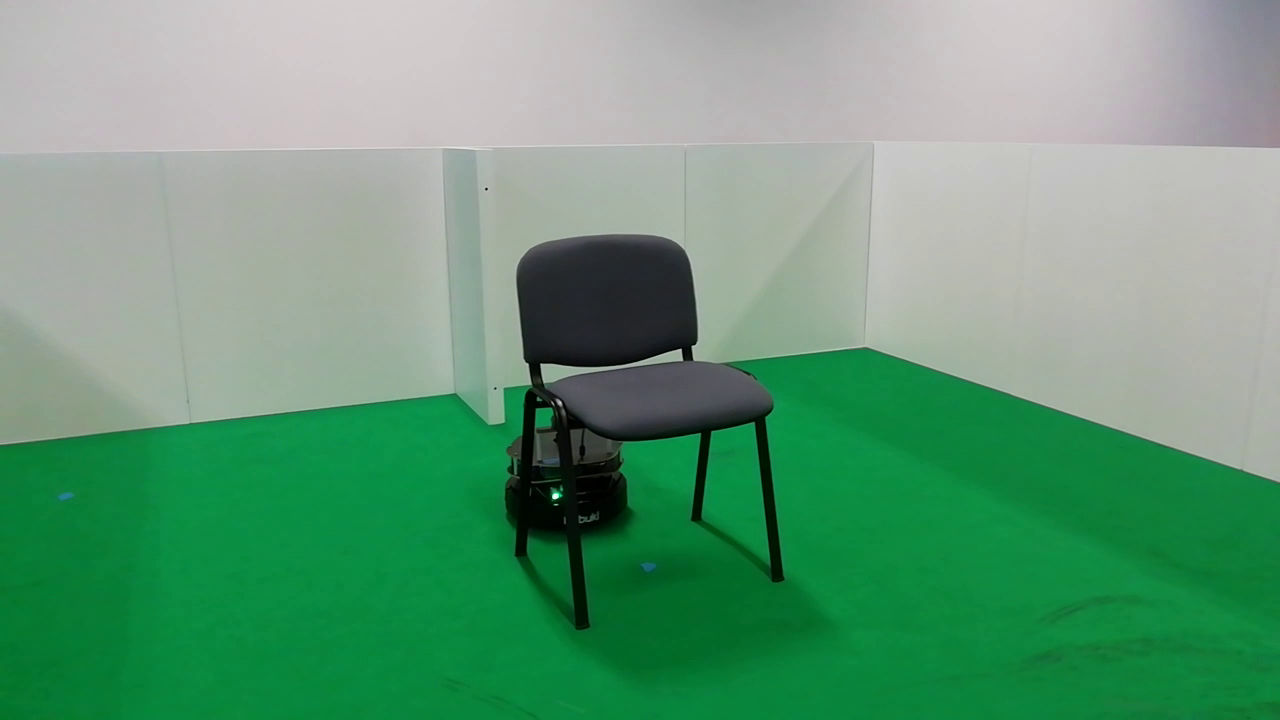
\includegraphics[width=\linewidth]{imgs/chapter5/nchairLF.png}
     \caption{Robot getting stuck in chair number 1}
     \label{fig::wchair}
  \end{subfigure}
  \begin{subfigure}[b]{0.49\linewidth}
    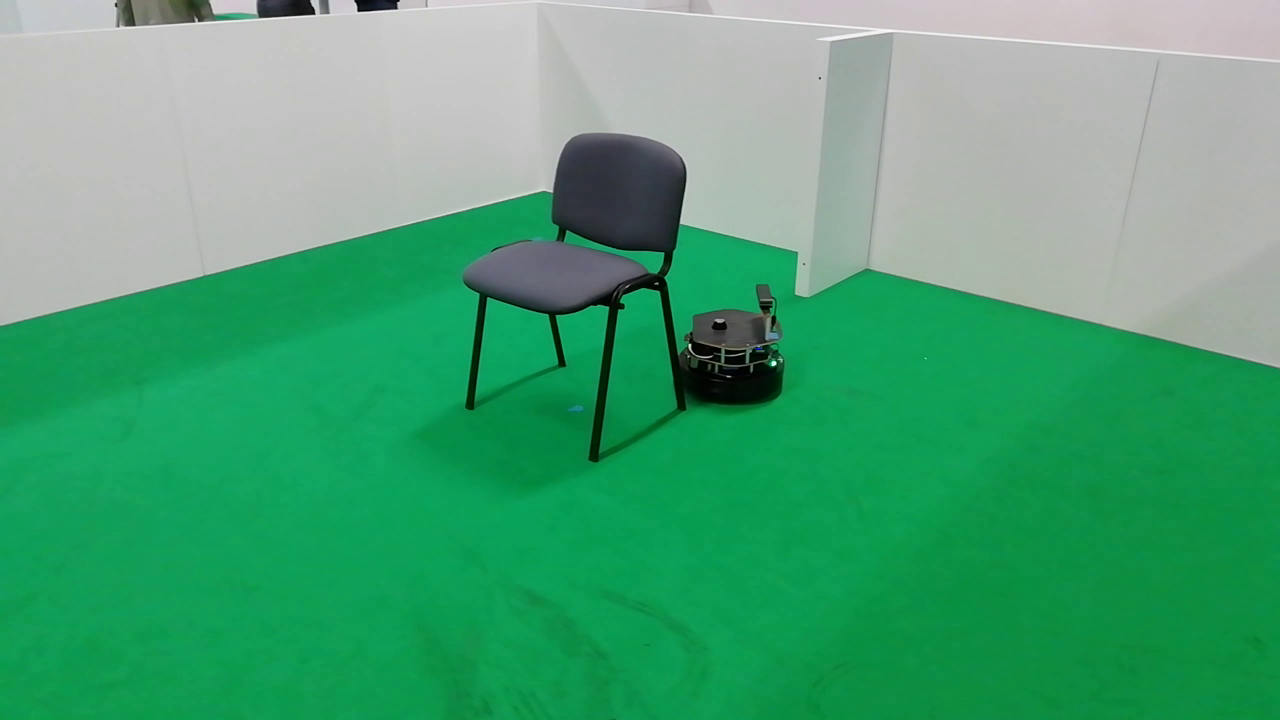
\includegraphics[width=\linewidth]{imgs/chapter5/nchairLF2.png}
    \caption{Robot getting stuck in chair number 2}
    \label{fig::nchair}
  \end{subfigure}
  \caption{Robot avoiding getting stuck in four legged chair}
  \label{fig:nchairLF}
\end{figure}

\subsubsection*{FMCW radar}
Using the \ac{FMCW} radar proved to be much better with the robot safely circumventing around the chair with safe distance for all duration of the task. Figure \ref{fig:nchairRS} shows two instances of the turtlebot avoiding the chair in at a safe distance.
\begin{figure}[h!]
  \centering
  \begin{subfigure}[b]{0.49\linewidth}
    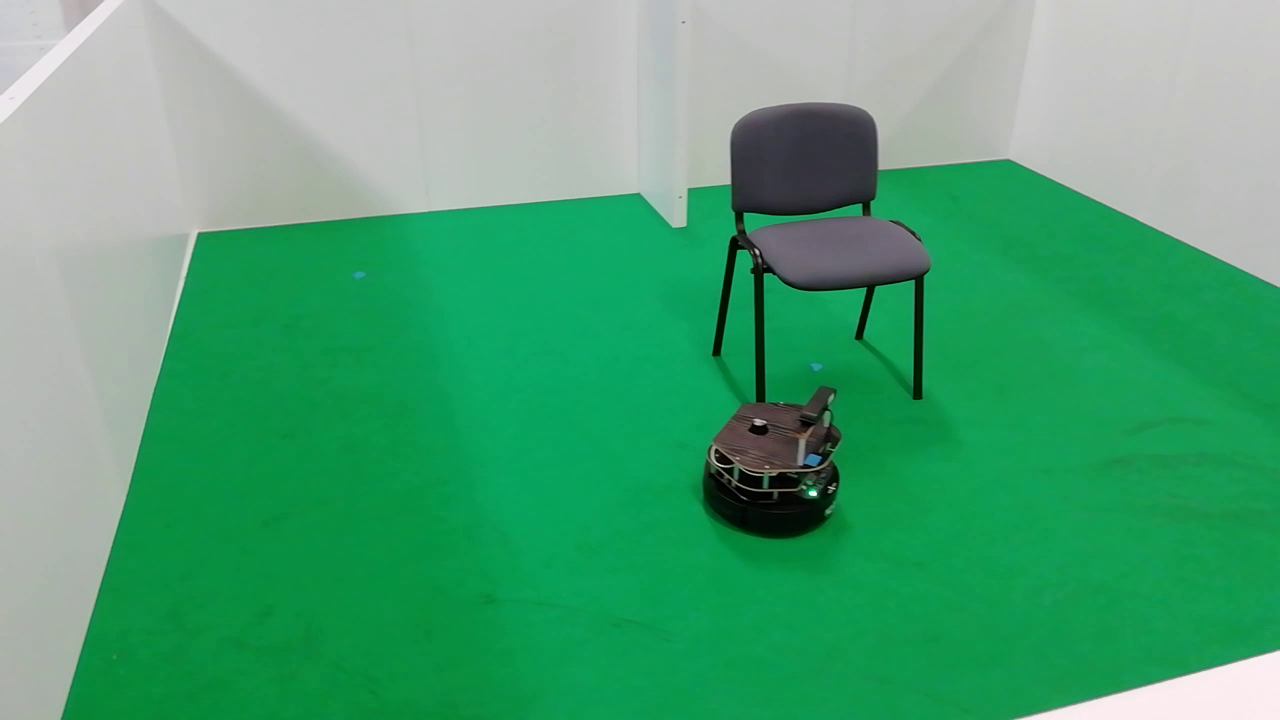
\includegraphics[width=\linewidth]{imgs/chapter5/nchairRS.png}
     \caption{Robot avoiding four legged chair number 1}
     \label{fig::wchair}
  \end{subfigure}
  \begin{subfigure}[b]{0.49\linewidth}
    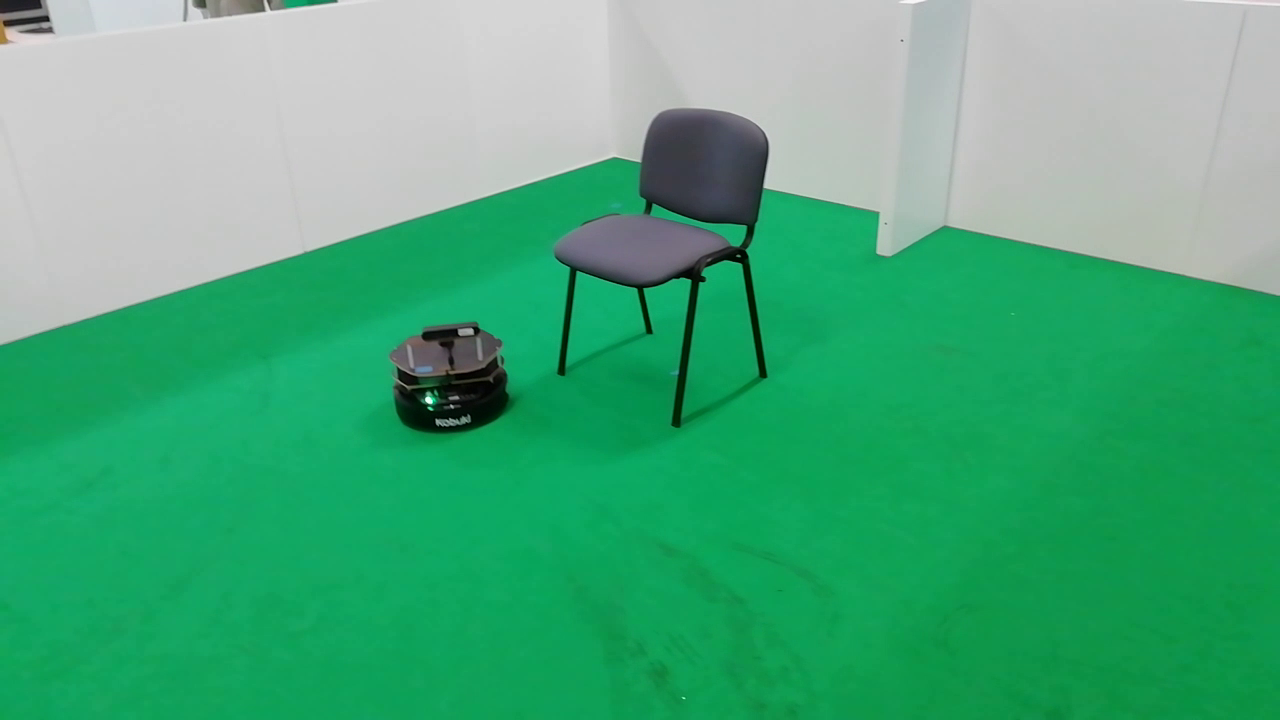
\includegraphics[width=\linewidth]{imgs/chapter5/nchairRS2.png}
    \caption{Robot avoiding four legged chair number 2}
    \label{fig::nchair}
  \end{subfigure}
  \caption{Robot avoiding the four legged chair}
  \label{fig:nchairRS}
\end{figure}

Analysing the data we see that when the robot is facing it it detects almost all legs immediately. 
%PUT RVIZ PICTURE?
This makes it so the robot is aware of it at all times and planning around it.


\subsubsection*{Robot Trajectory}

Figure \ref{fig:traj2} shows the trajectory of the robot for the \ac{LiDAR} and \ac{FMCW} \ac{radar} and an approximate position of the invalid space the four legs of the chair create coloured in dimmed red. The center of the robot should not passtrough this area since it will lead to collision. As we can see the trajectory  produced in the \ac{FMCW} radar case is much less susceptible to the object than in the \ac{LiDAR} case. 
\begin{figure}[ht!]
\centerline{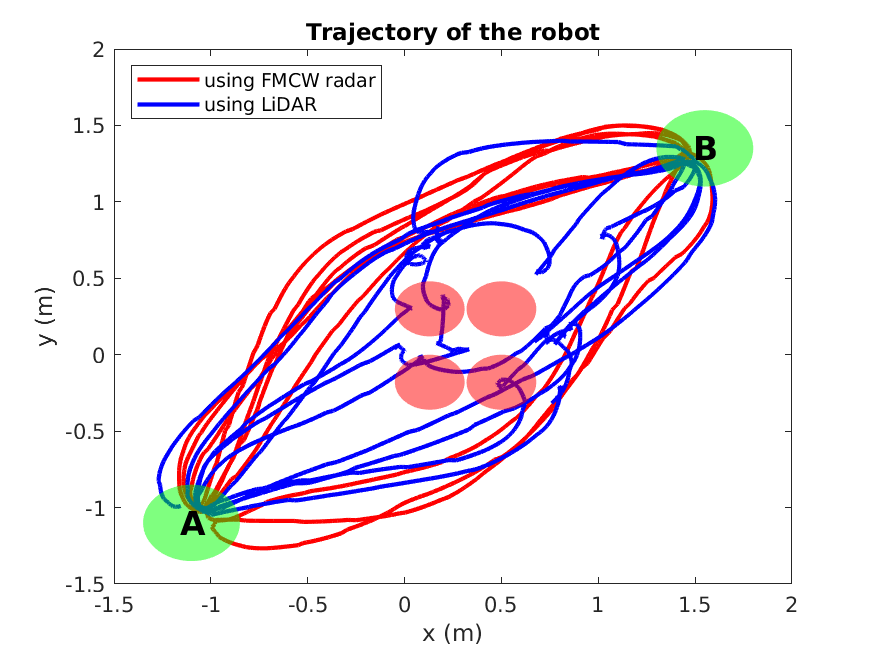
\includegraphics [width=0.7 \textwidth]{imgs/chapter5/traj2.png}}
\caption{Trajectory of the robot for the four-legged chair's case}
\label{fig:traj2}
\end{figure}

\subsubsection{Garbage Bin}

\subsubsection*{LiDAR}
In this case the robot went in a straight line as in the wheeled chair's case pushing the garbage bin until it reached its first goal. This happened again because the \ac{LiDAR} was unable to properly detect the garbage bin at a certain angle.  Figure \ref{fig:garbageLF} shows two instances of the turtlebot hitting the garbage bin.
\begin{figure}[h!]
  \centering
  \begin{subfigure}[b]{0.49\linewidth}
    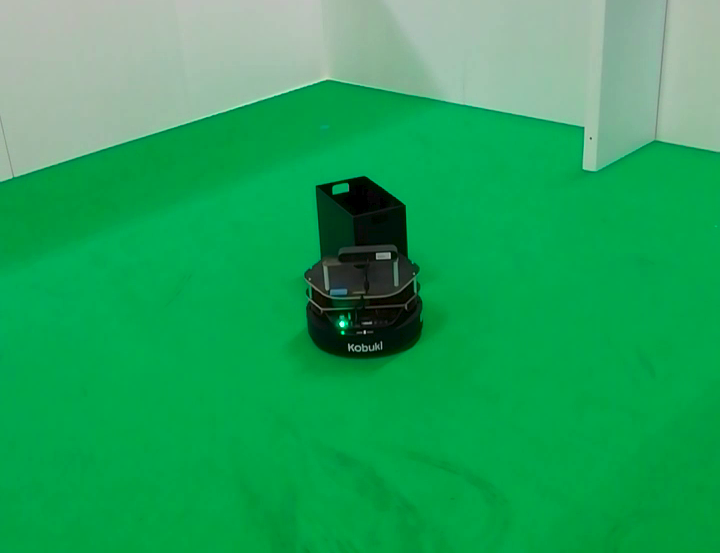
\includegraphics[width=\linewidth]{imgs/chapter5/garbageLF.png}
     \caption{Robot crashing into garbage bin}
     \label{fig:garbageLF1}
  \end{subfigure}
  \begin{subfigure}[b]{0.49\linewidth}
    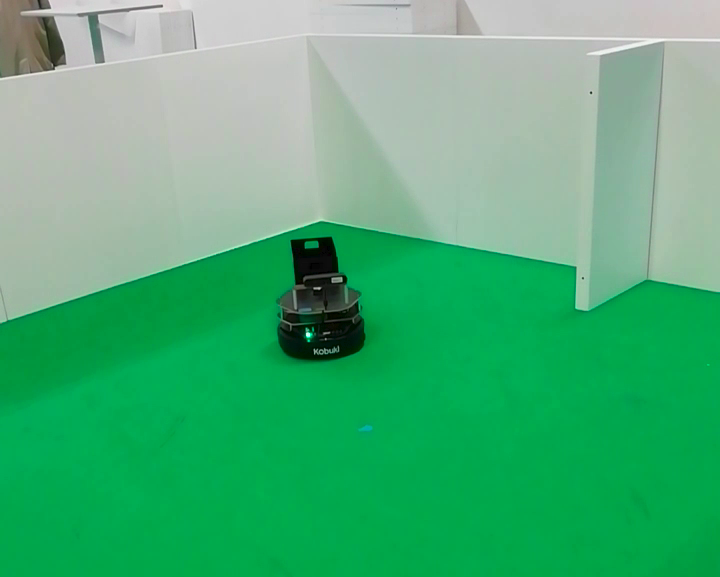
\includegraphics[width=\linewidth]{imgs/chapter5/garbageLF2.png}
    \caption{Robot pushing garbage bin}
    \label{fig:garbageLF2}
  \end{subfigure}
  \caption{Two instances of the robot's navigation with the garbage bin as an obstacle}
  \label{fig:garbageLF}
\end{figure}



\subsubsection*{FMCW radar}
Using the \ac{FMCW} radar the robot did detect it properly and went around it easily.
 Figure \ref{fig:garbageRS} shows two instances of the turtlebot avoiding the garbage bin at a safe distance.
\begin{figure}[h!]
  \centering
  \begin{subfigure}[b]{0.49\linewidth}
    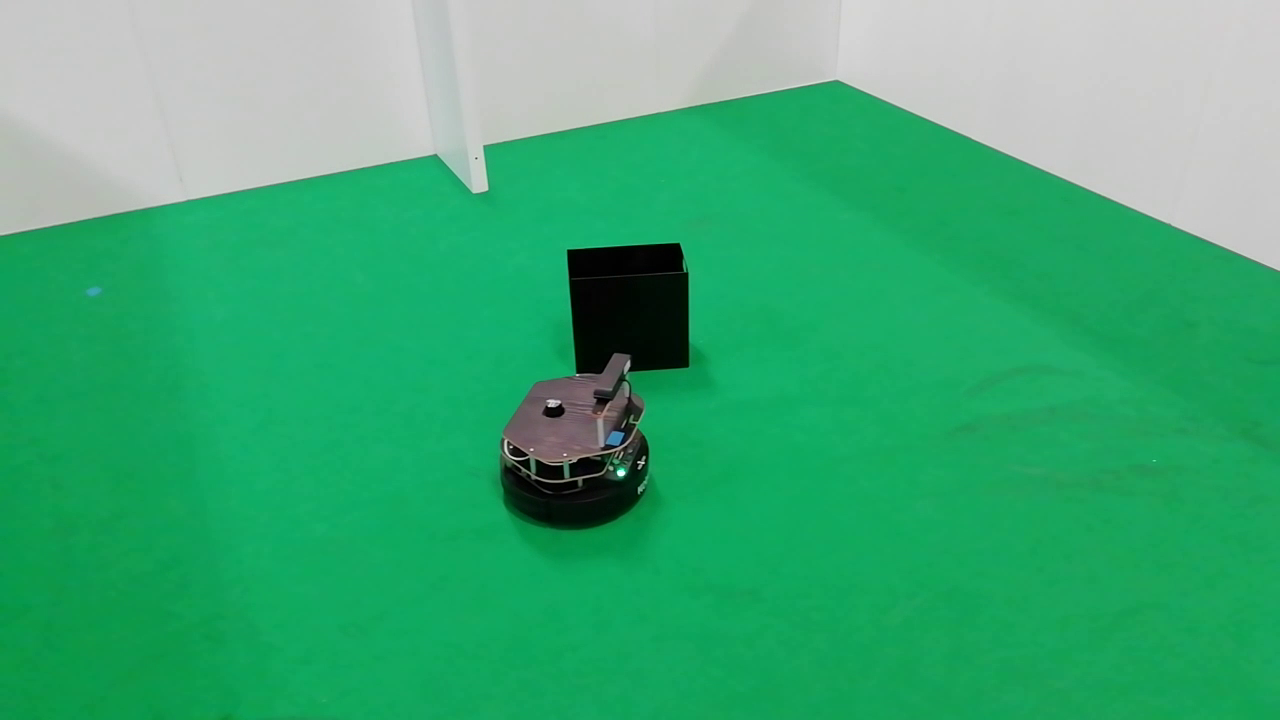
\includegraphics[width=\linewidth]{imgs/chapter5/garbageRS.png}
     \caption{Robot avoiding garbage bin number 1}
     \label{fig::wchair}
  \end{subfigure}
  \begin{subfigure}[b]{0.49\linewidth}
    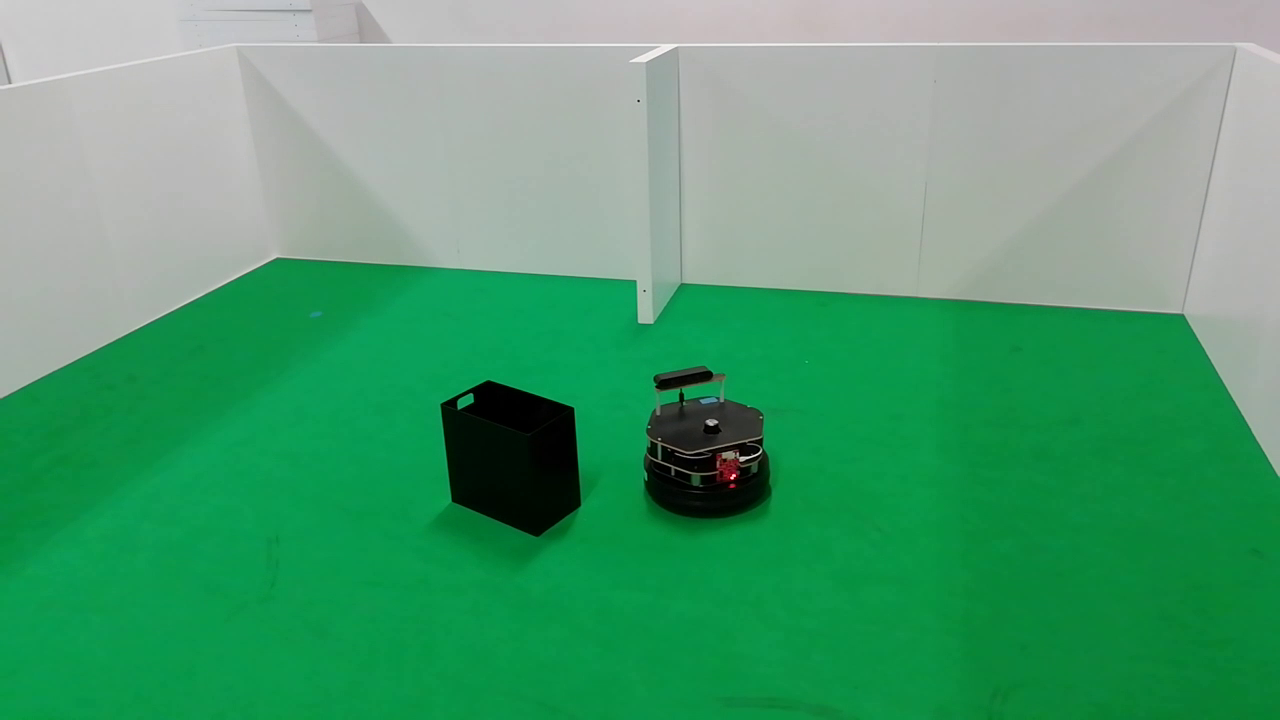
\includegraphics[width=\linewidth]{imgs/chapter5/garbageRS2.png}
    \caption{Robot avoiding garbage bin  number 2}
    \label{fig::nchair}
  \end{subfigure}
  \caption{Robot avoiding garbage bin}
  \label{fig:garbageRS}
\end{figure}

\subsubsection{Box}
\subsubsection*{LiDAR}
In the LiDAR's case the robot did not detect the low height box throughout all the course. This makes sense since the this sensor is built to detect objects that are the same height as the sensor. In other words it is optimized to detect only the horizontal plane of the 2D-\ac{LiDAR}. This failure of detection made it so the robot could not replan its course and in consequence it collided with said box. Figure \ref{fig::boxLF} shows two instances where the robot collided with the box using \ac{LiDAR} as a sensor source.

\begin{figure}[h!]
  \centering
  \begin{subfigure}[b]{0.49\linewidth}
    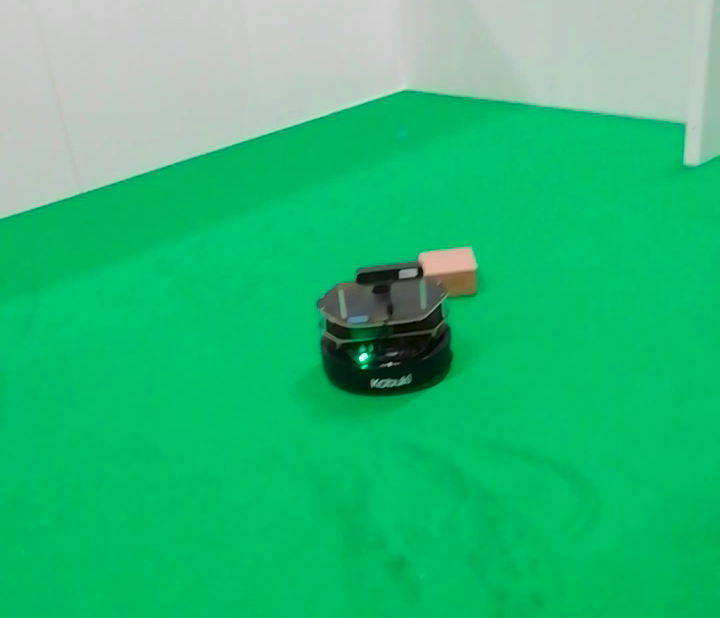
\includegraphics[width=\linewidth]{imgs/chapter5/boxLF.png}
     \caption{Robot collision with box number 1}
     \label{fig::box}
  \end{subfigure}
  \begin{subfigure}[b]{0.46\linewidth}
    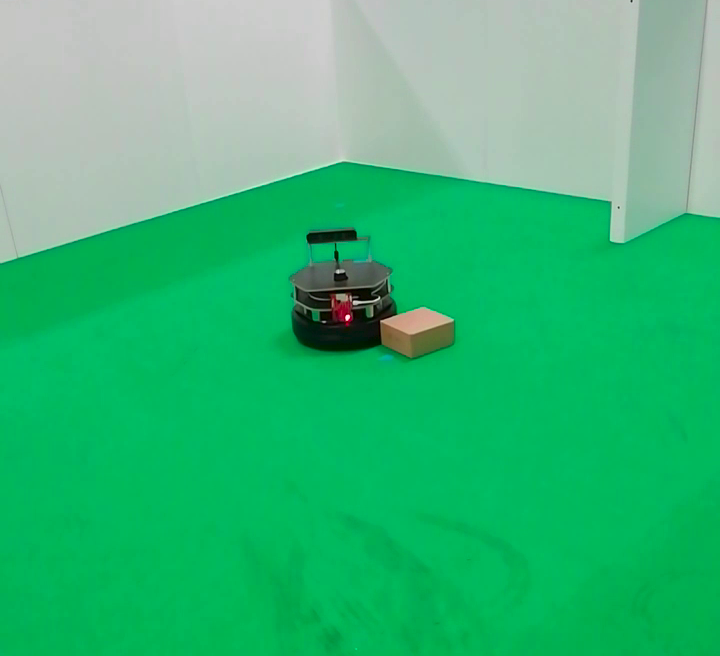
\includegraphics[width=\linewidth]{imgs/chapter5/boxLF2.png}
    \caption{Robot collision with box number 2}
    \label{fig::box}
  \end{subfigure}
  \caption{Robot collision with box}
  \label{fig::boxLF}
\end{figure}


\subsubsection*{FMCW radar}
For this case initially the robot also did not detect the box. However by decreasing the threshold of the passthrough filter of intensity to 14 we made it so it can detect it. With this modification the robot was able to complete the test without colliding with the box. Figure \ref{fig:boxRS} shows two instances of the robot performing the course avoiding the box with the previous modification. However this change may result in the \ac{FMCW} \ac{radar} having false detections due to now having a lower level of \ac{SNR}.

\begin{figure}[ht!]
  \centering
  \begin{subfigure}[b]{0.4\linewidth}
    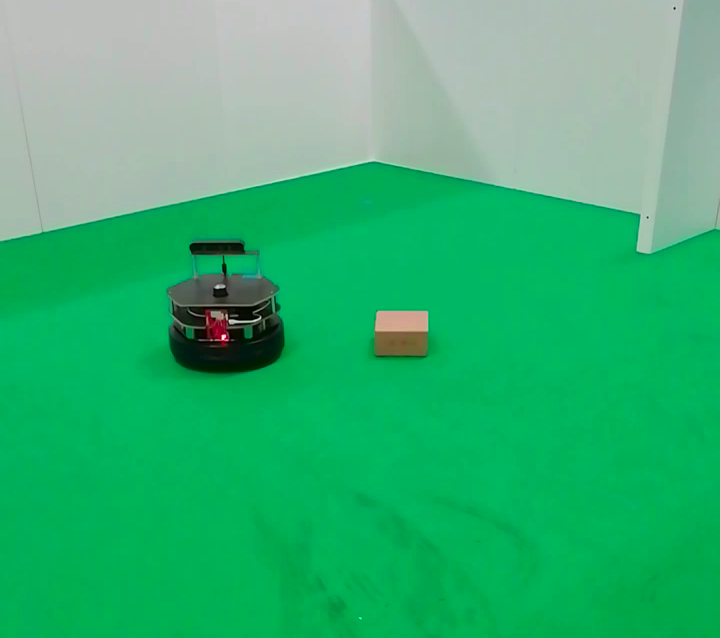
\includegraphics[width=\linewidth]{imgs/chapter5/boxRS.png}
     \caption{Robot avoiding box number 1}
     \label{fig::wchair}
  \end{subfigure}
  \begin{subfigure}[b]{0.38\linewidth}
    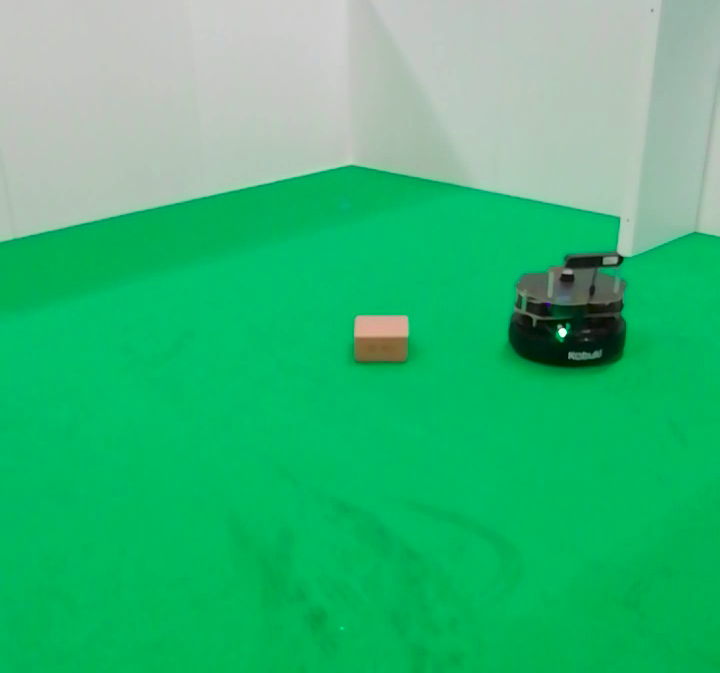
\includegraphics[width=\linewidth]{imgs/chapter5/boxRS2.png}
    \caption{Robot avoiding box  number 2}
    \label{fig::nchair}
  \end{subfigure}
  \caption{Robot avoiding box}
  \label{fig:boxRS}
\end{figure}

\subsubsection{Acrylic tube}

\subsubsection*{LiDAR}
When it comes to the Acrylic tube using the 2-D \ac{LiDAR} it falsely detected targets where there where none. This is due to the physical proprieties of the object being unsuitable for \ac{LiDAR} technology to handle. The robot in its course got stuck near the obstacle due to thinking it had crashed into it. However this was not the case and the robot did not succeed in the experiment. Figure \ref{fig:glassRS} shows two instances of the robot getting stuck in the acrylic tube.

\begin{figure}[ht!]
  \centering
  \begin{subfigure}[b]{0.49\linewidth}
    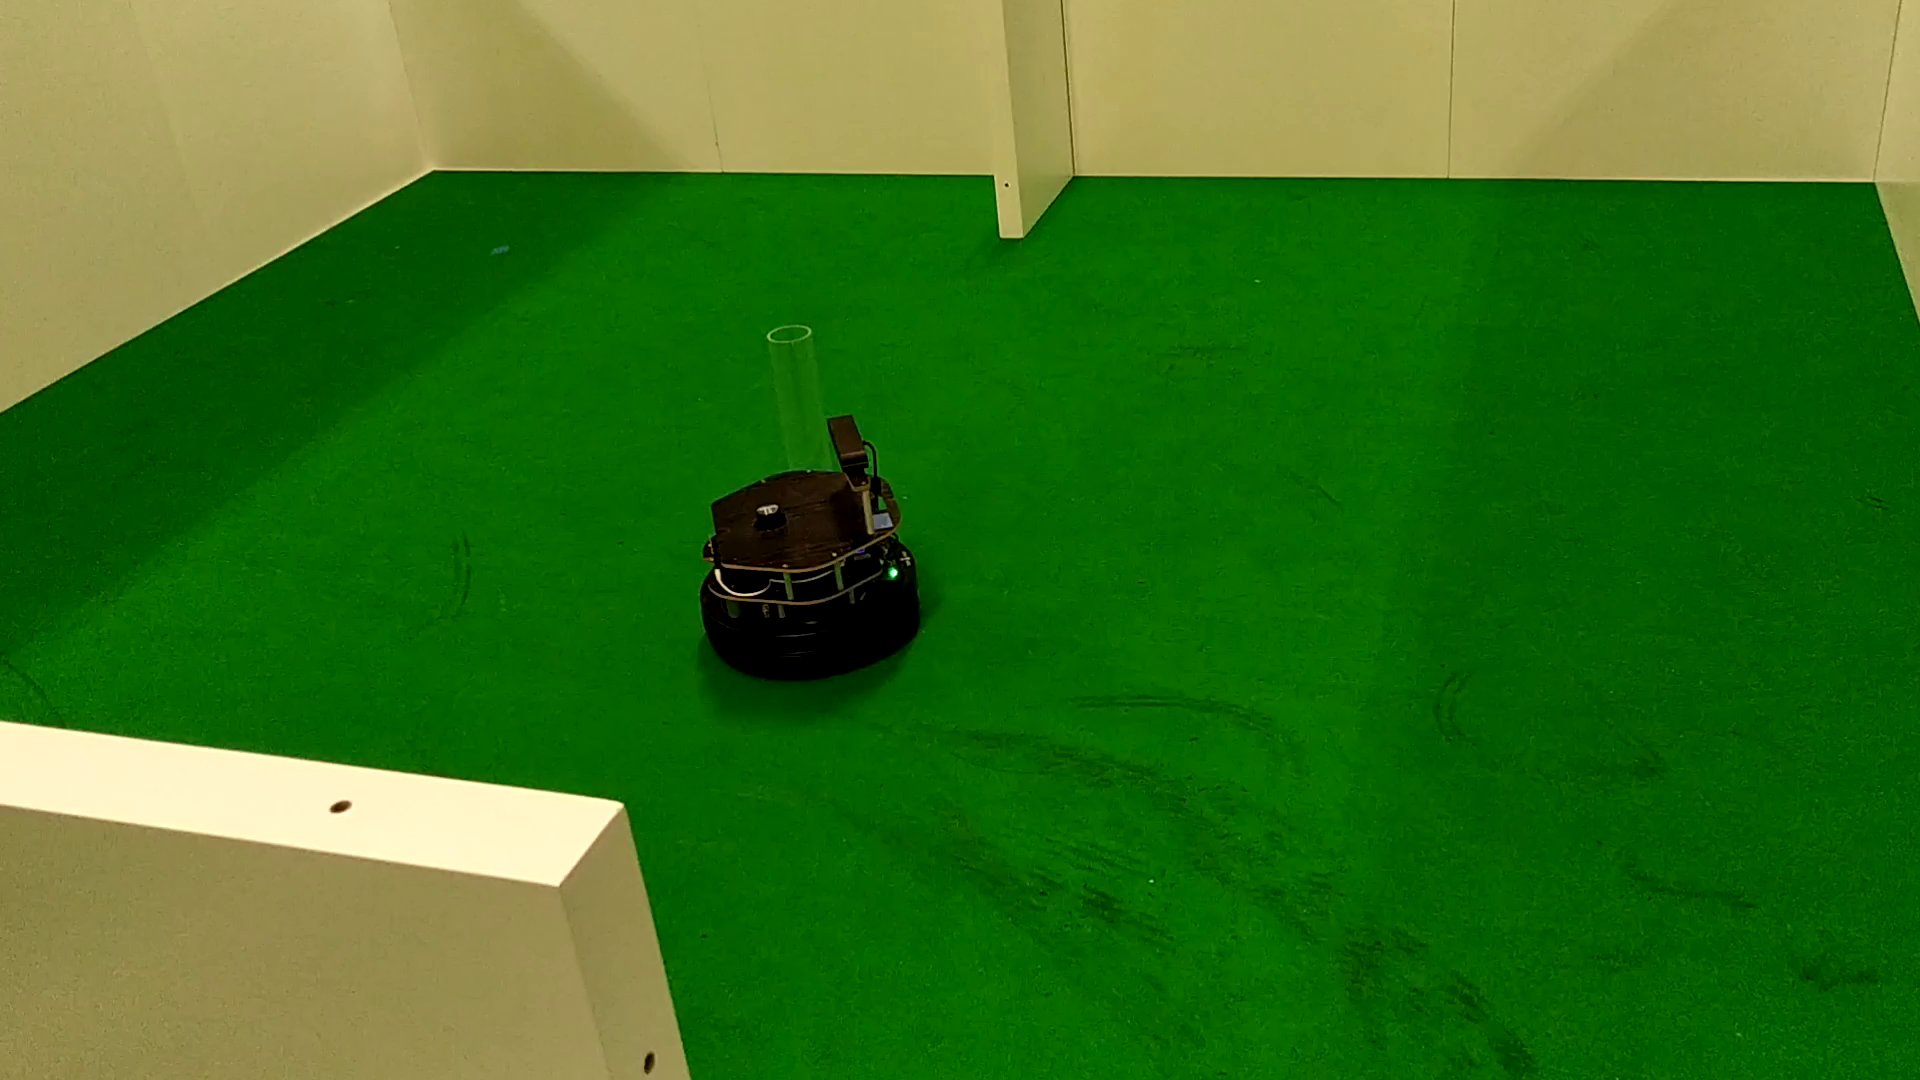
\includegraphics[width=\linewidth]{imgs/chapter5/glassLF1.png}
     \caption{Robot getting stuck acrylic tube number 1}
     \label{fig::glassRS1}
  \end{subfigure}
  \begin{subfigure}[b]{0.49\linewidth}
    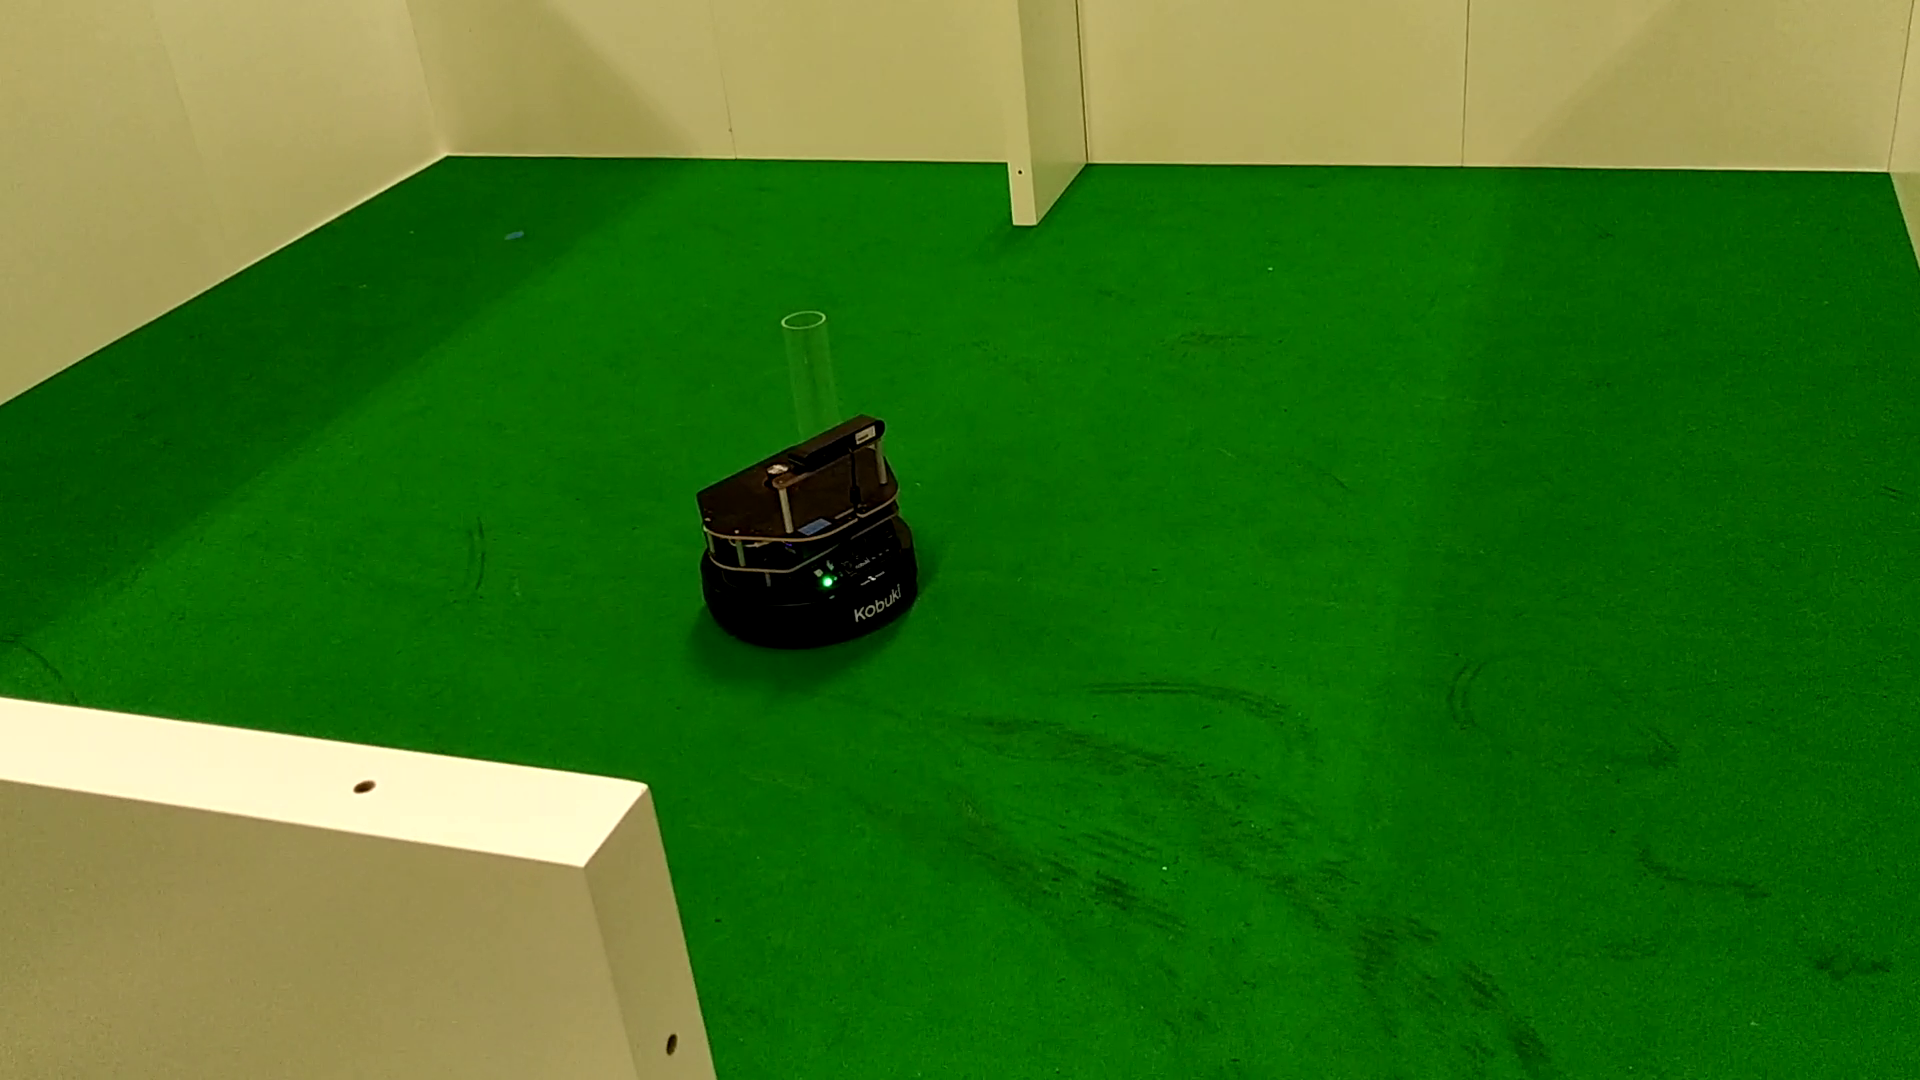
\includegraphics[width=\linewidth]{imgs/chapter5/glassLF2.png}
    \caption{Robot getting stuck in acrylic tube  number 2}
    \label{fig::glassRS2}
  \end{subfigure}
  \caption{Robot getting stuck in acrylic tube}
  \label{fig:glassRS}
\end{figure}

\subsubsection*{FMCW radar}
In this case the robot was able to properly detect the tube and with it avoided it through all the course. The behavior of the robot was objectively better than the previous case since it went through all course without hitting the tube in any way. Figure \ref{fig:glassRS} shows two instances of the robot avoiding the acrylic tube.

\begin{figure}[ht!]
  \centering
  \begin{subfigure}[b]{0.49\linewidth}
    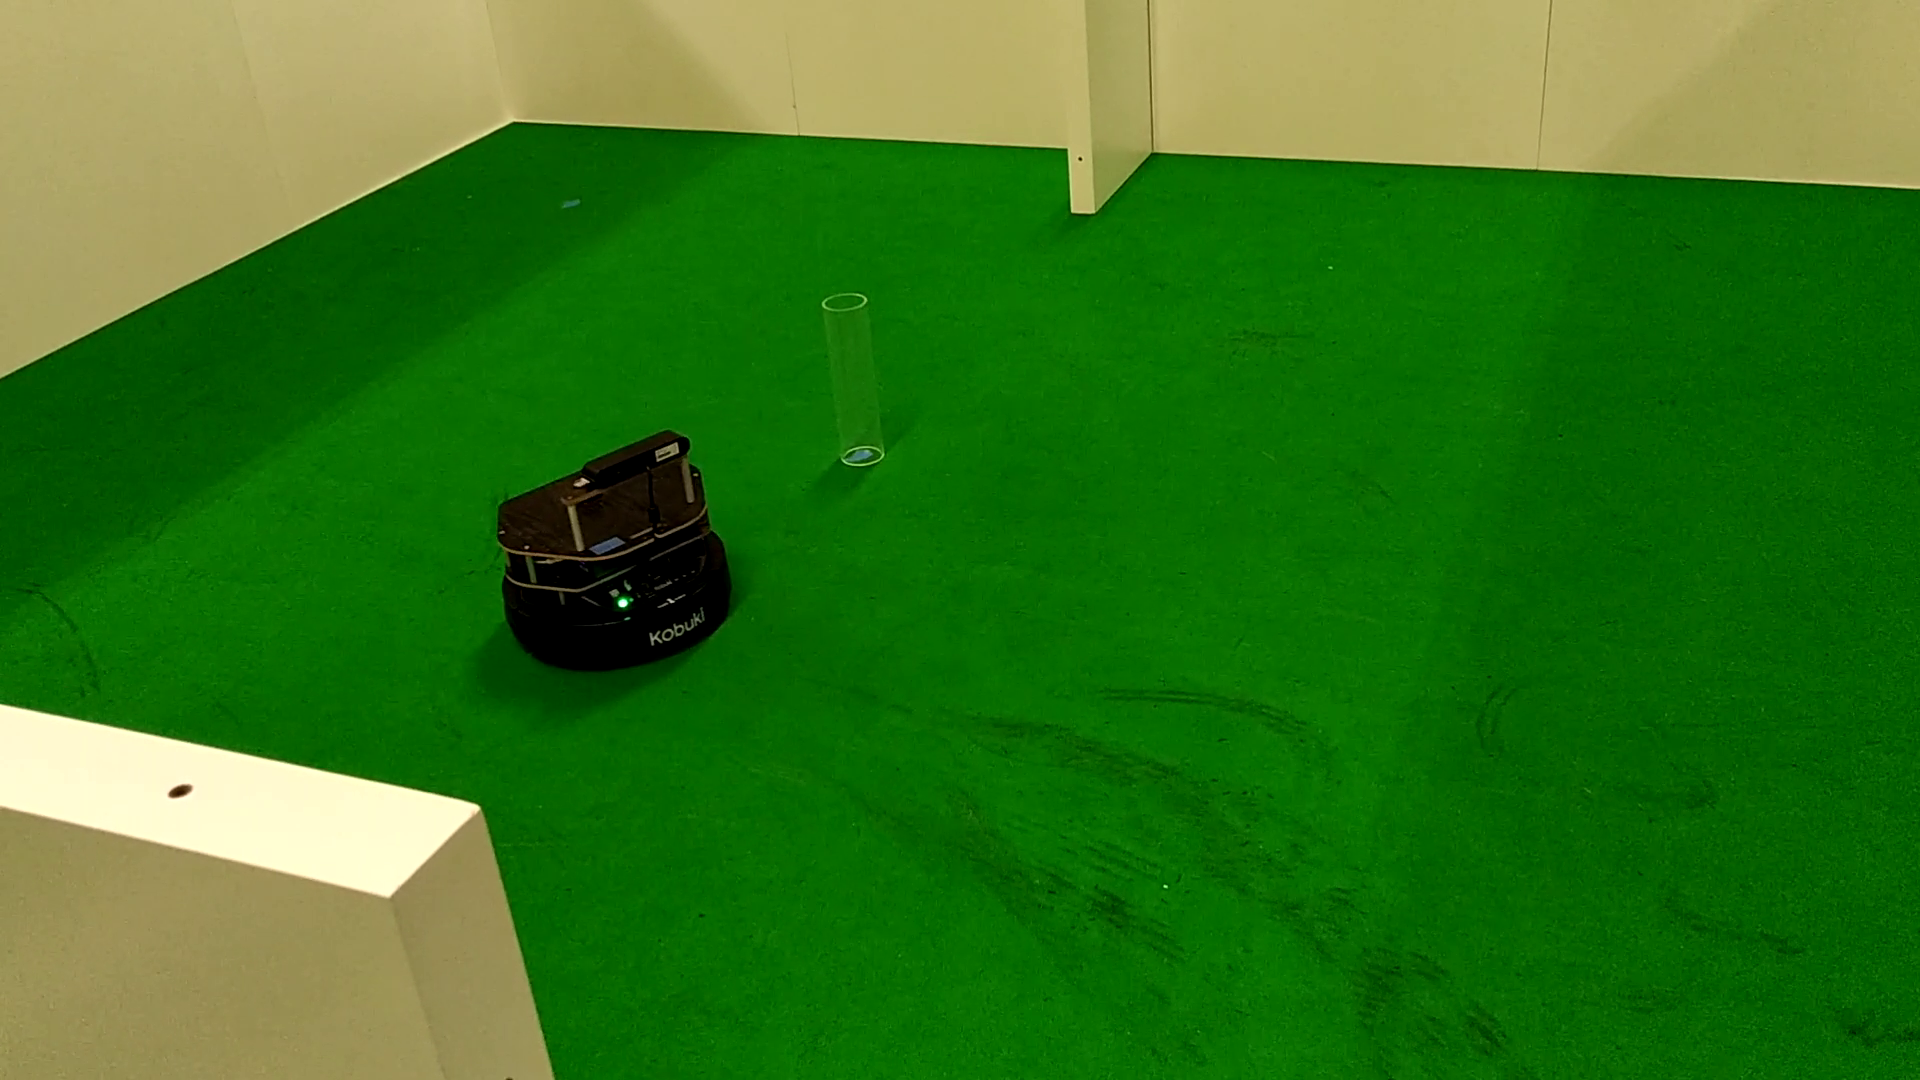
\includegraphics[width=\linewidth]{imgs/chapter5/glassRS1.png}
     \caption{Robot avoiding acrylic tube number 1}
     \label{fig::glassRS1}
  \end{subfigure}
  \begin{subfigure}[b]{0.49\linewidth}
    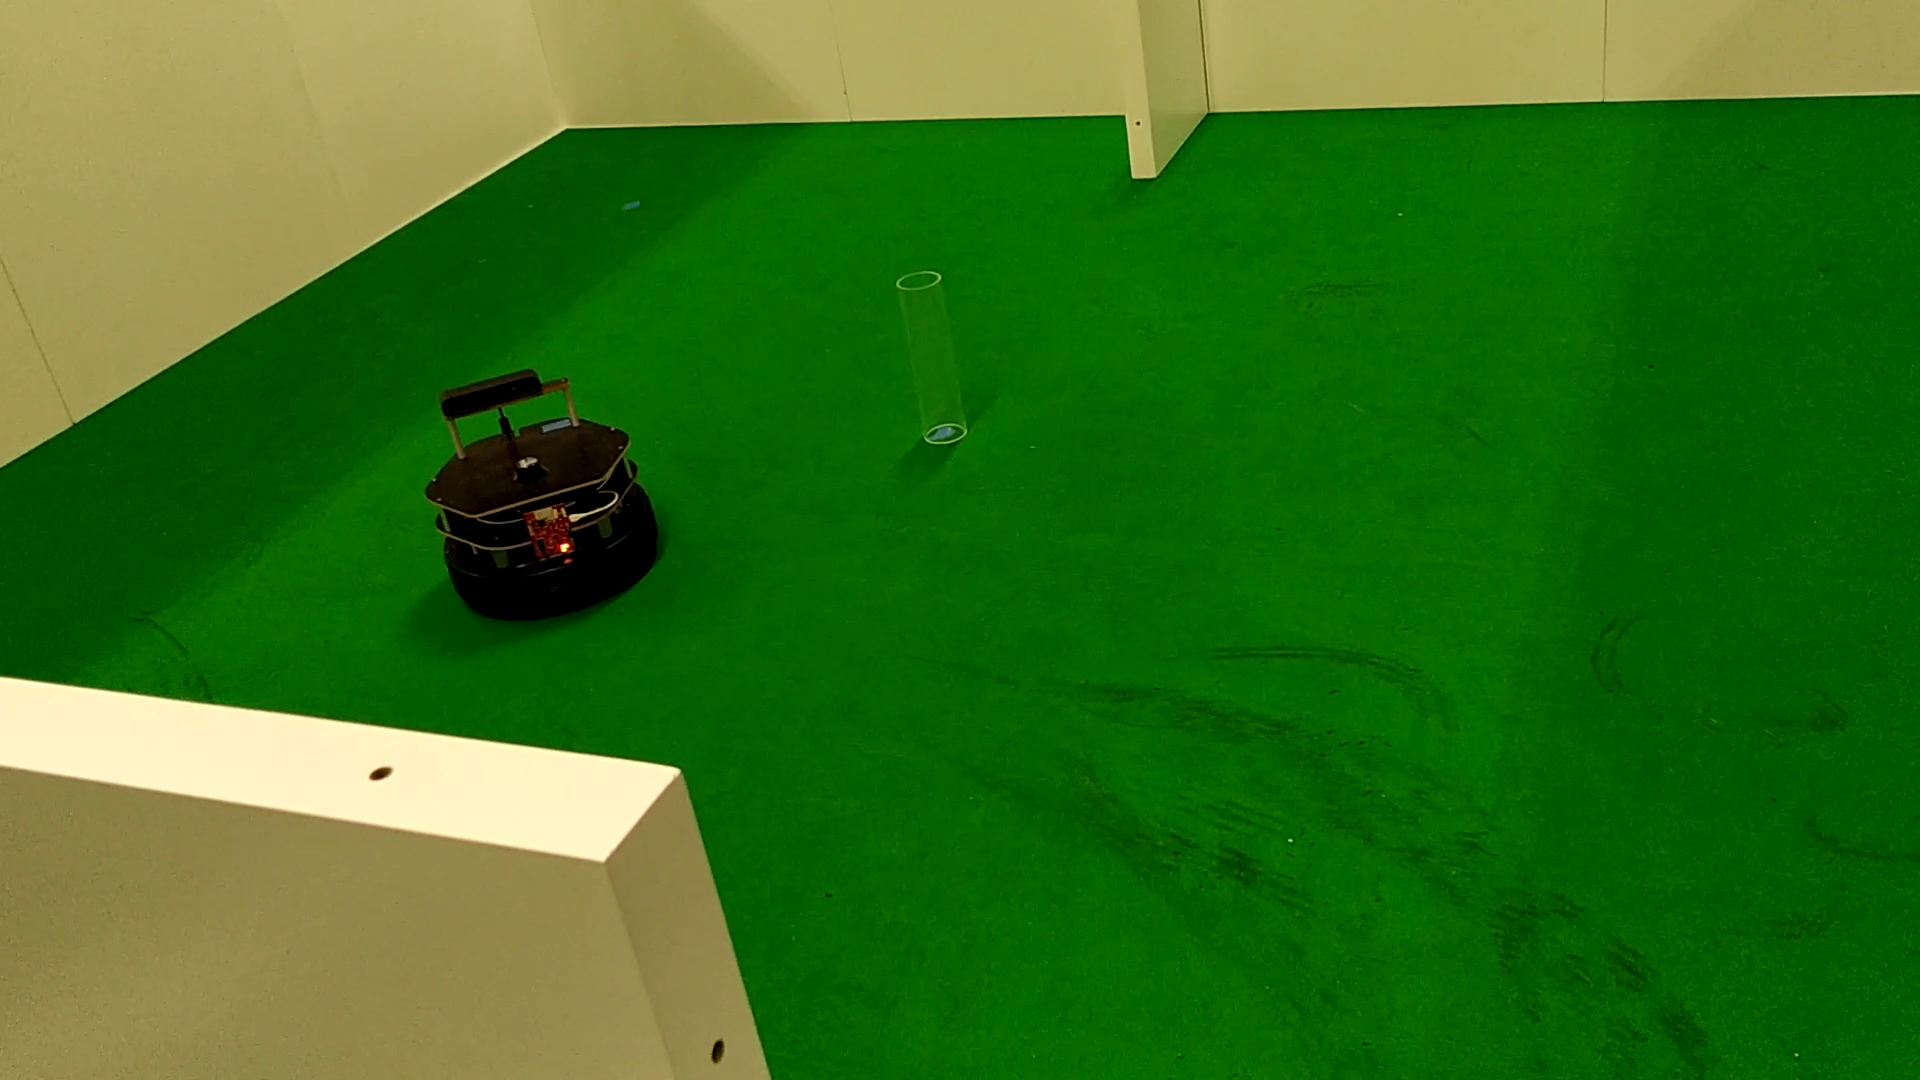
\includegraphics[width=\linewidth]{imgs/chapter5/glassRS2.png}
    \caption{Robot avoiding acrylic tube  number 2}
    \label{fig::glassRS2}
  \end{subfigure}
  \caption{Robot avoiding acrylic tube box}
  \label{fig:glassRS}
\end{figure}

\subsubsection{Robot  (turtlebot2) }
In this last case both the \ac{FMCW} \ac{radar} and the 2D-LIDAR performed reasonably well avoiding the obstacle with ease for all the trajectory.

\subsection{Discussion}
In this experiment we conclude that there are multiple types of obstacles that the 2-D LiDAR is unable to properly detect. This poor detection led to the robot crashing into the objects making it so the navigation task presented ended in failure. However using the \ac{FMCW} radar proved to have a better perception of all the obstacles in the experiment and with it the indoor navigation tests were concluded with success with the robot circumventing them in a safe manner.


\section{Dynamic Obstacles in controlled environment}
In the previous experiment we only dealt with static objects however in this new test we want to see how the robot handles dynamic objects in a controlled space. For that we send multiple goals  to the robot and use an additional turtlebot2 or a person to obstruct its path. In other words we have the robot trying to reach multiple goals multiple times and the dynamic obstacle will try to make more difficult by obstructing the planned paths of the robot.  The main goal of this experiment is to see if the robot can handle unstructured environments that are often the case in indoor scenarios.
\subsection{Experimental Setup}
For this test we send four goals to the robotic platform, A,B,C and D in zigzag fashion and we will place a dynamic obstacle obstructing it as shown in Figure \ref{fig:exp3}.

\begin{figure}[ht!]
\centerline{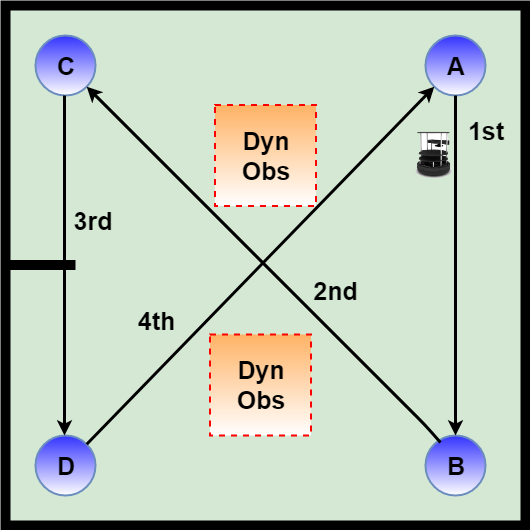
\includegraphics [width=0.5 \textwidth]{imgs/chapter5/exp3.png}}
\caption[Demonstration of the course of test]{Demonstration of the course of test, the robot will run through A-B-C-D  while  trying to avoid the dynamic obstacle obstructing its path}
\label{fig:exp3}
\end{figure}
For the dynamic obstacles we will use first person and in a second trial a a mobile robot. This obstacles will try to obstruct the path of the robot throughout the course. For this case we will only use the \ac{FMCW} \ac{radar} as an obstacle detector.


\subsection{Results}
In the following sections we show the results for the person and the mobile robot as obstacles for the experiment.
\subsubsection{Person}
Throughout all the test the robot was successfully avoided the person  only using the \ac{FMCW} \ac{radar} as an obstacle detector. Figure \ref{fig:exp3person} shows two instances of the the robot avoiding the person in the experiment.
\begin{figure}[ht!]
  \centering
  \begin{subfigure}[b]{0.49\linewidth}
    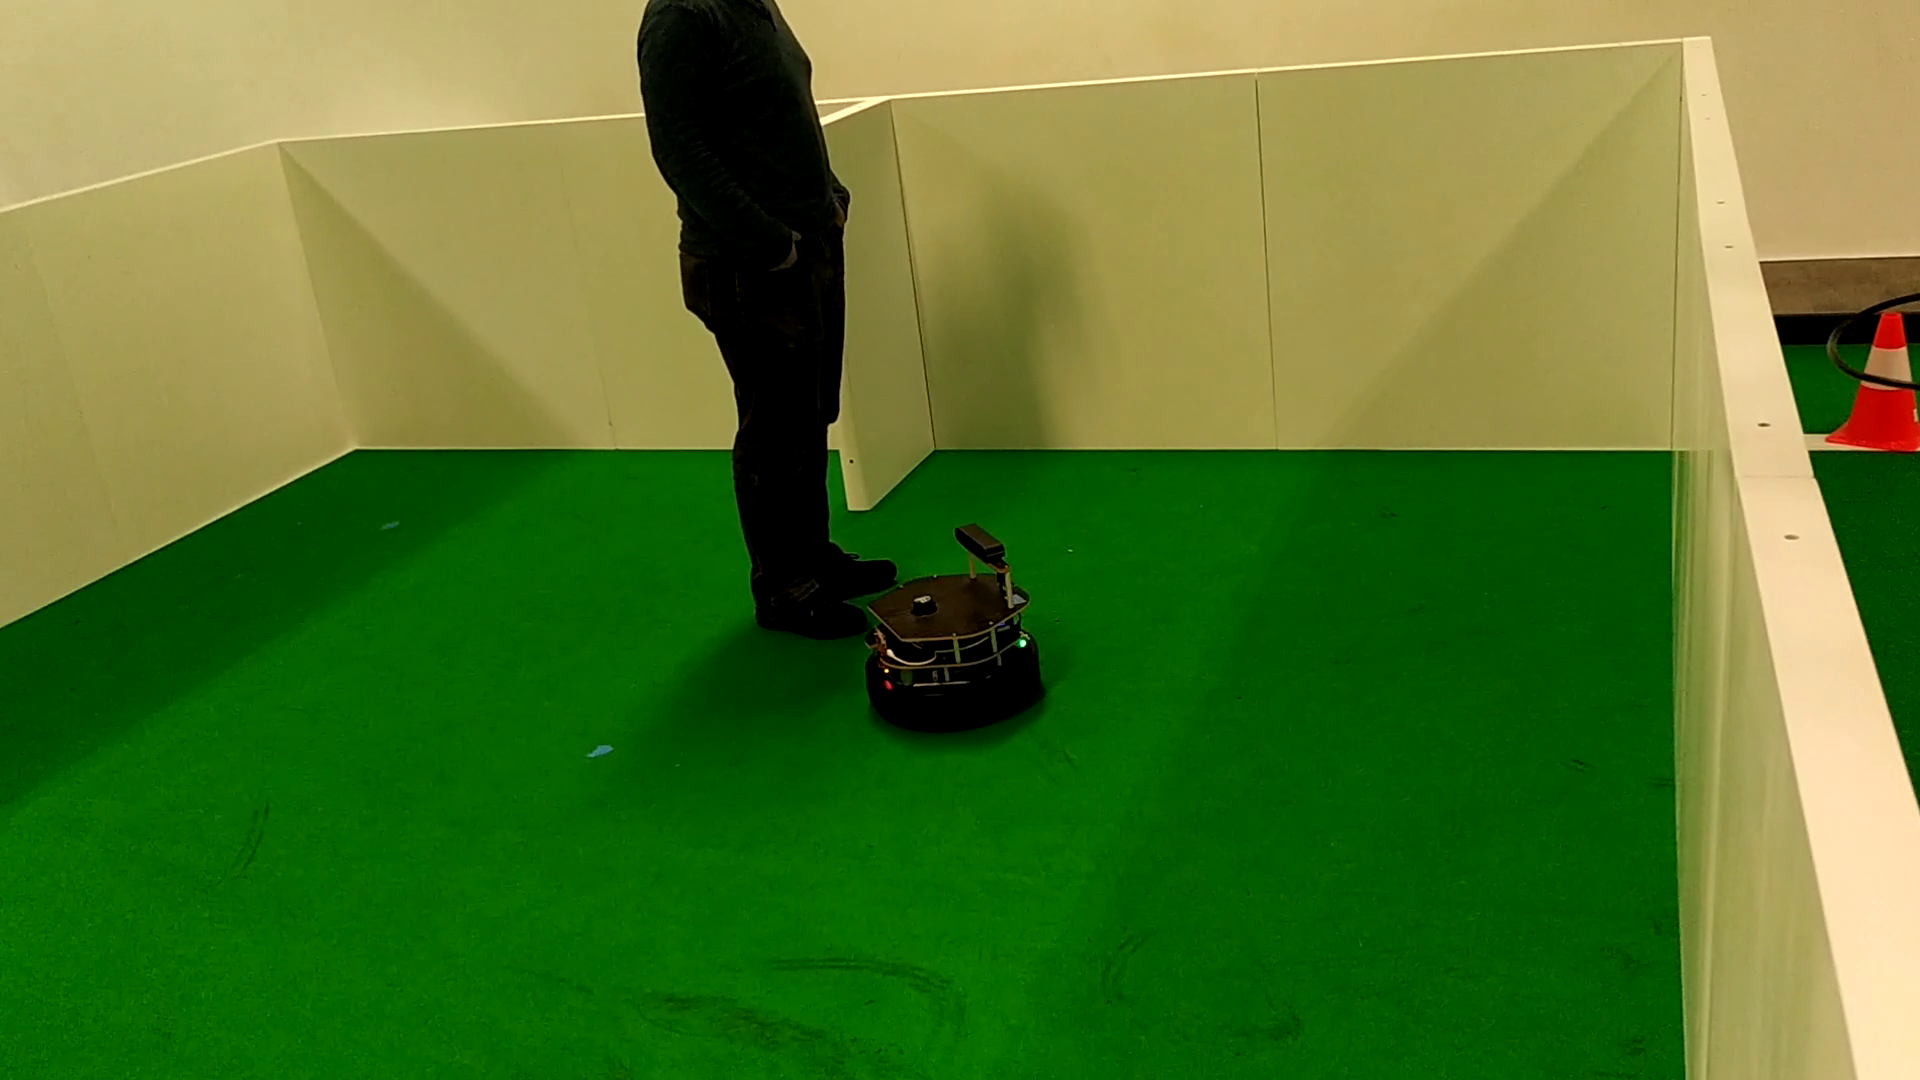
\includegraphics[width=\linewidth]{imgs/chapter5/exp3person1.png}
     \caption{Robot avoiding person number 1}
     \label{fig::exp3person1}
  \end{subfigure}
  \begin{subfigure}[b]{0.49\linewidth}
    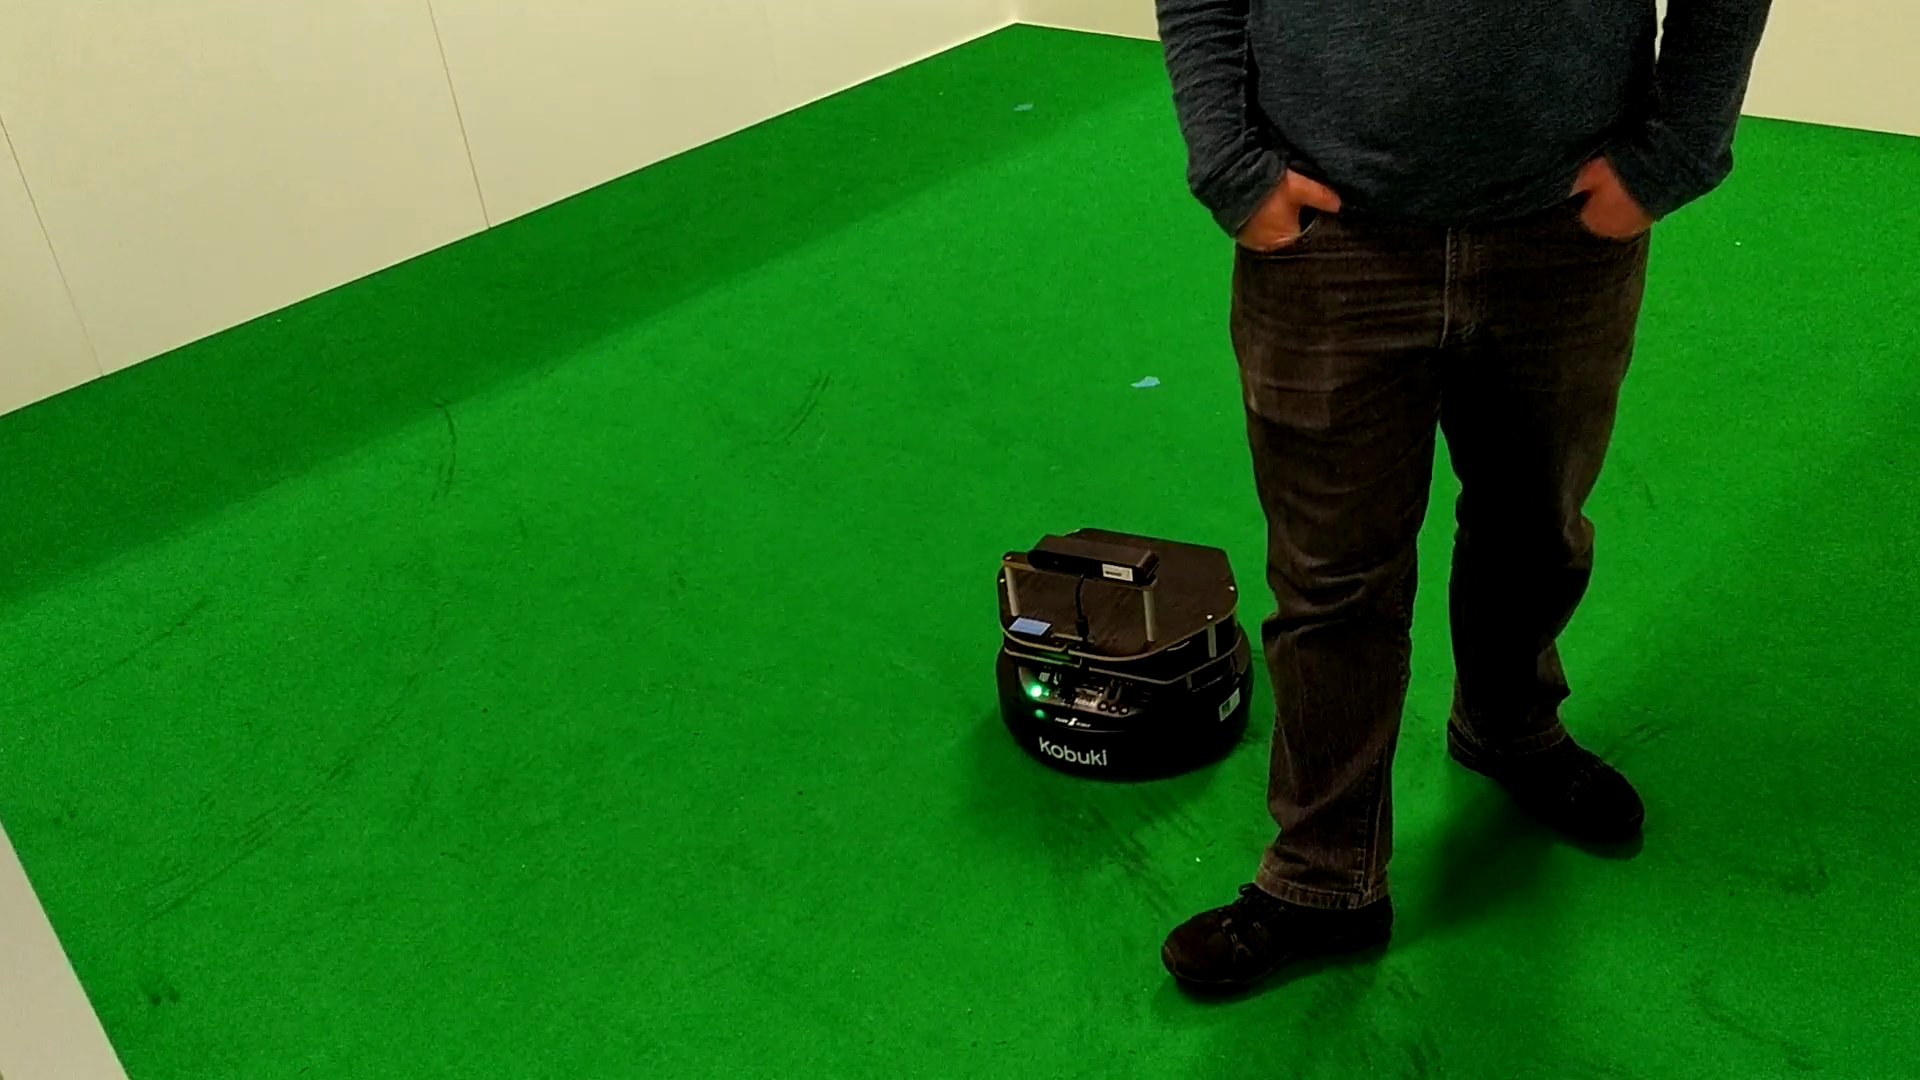
\includegraphics[width=\linewidth]{imgs/chapter5/exp3person2.png}
    \caption{Robot avoiding person  number 2}
    \label{fig::exp3person2}
  \end{subfigure}
  \caption{Robot avoiding person }
  \label{fig:exp3person}
\end{figure}
However the robot was only able to perceive the legs of said person and not its feet. This may lead to cases where the robot shocks in the person if it is to close.

When the person got to close to the robot, it stopped completely and had to recover behaviors were activated. We conclude that the \ac{FMCW} \ac{radar} is better suited for detecting obstacles that are at least half a meter away from the robot and that are facing it directly. 
\subsubsection{Mobile Robot}
For the mobile robot case the results were similar to the previous case. The robot was able to detect and avoid the the the other robot when it is facing him.

Figure \ref{fig:exp3robot} shows two instances of the robot avoiding the dynamic robot.
\begin{figure}[ht!]
  \centering
  \begin{subfigure}[b]{0.49\linewidth}
    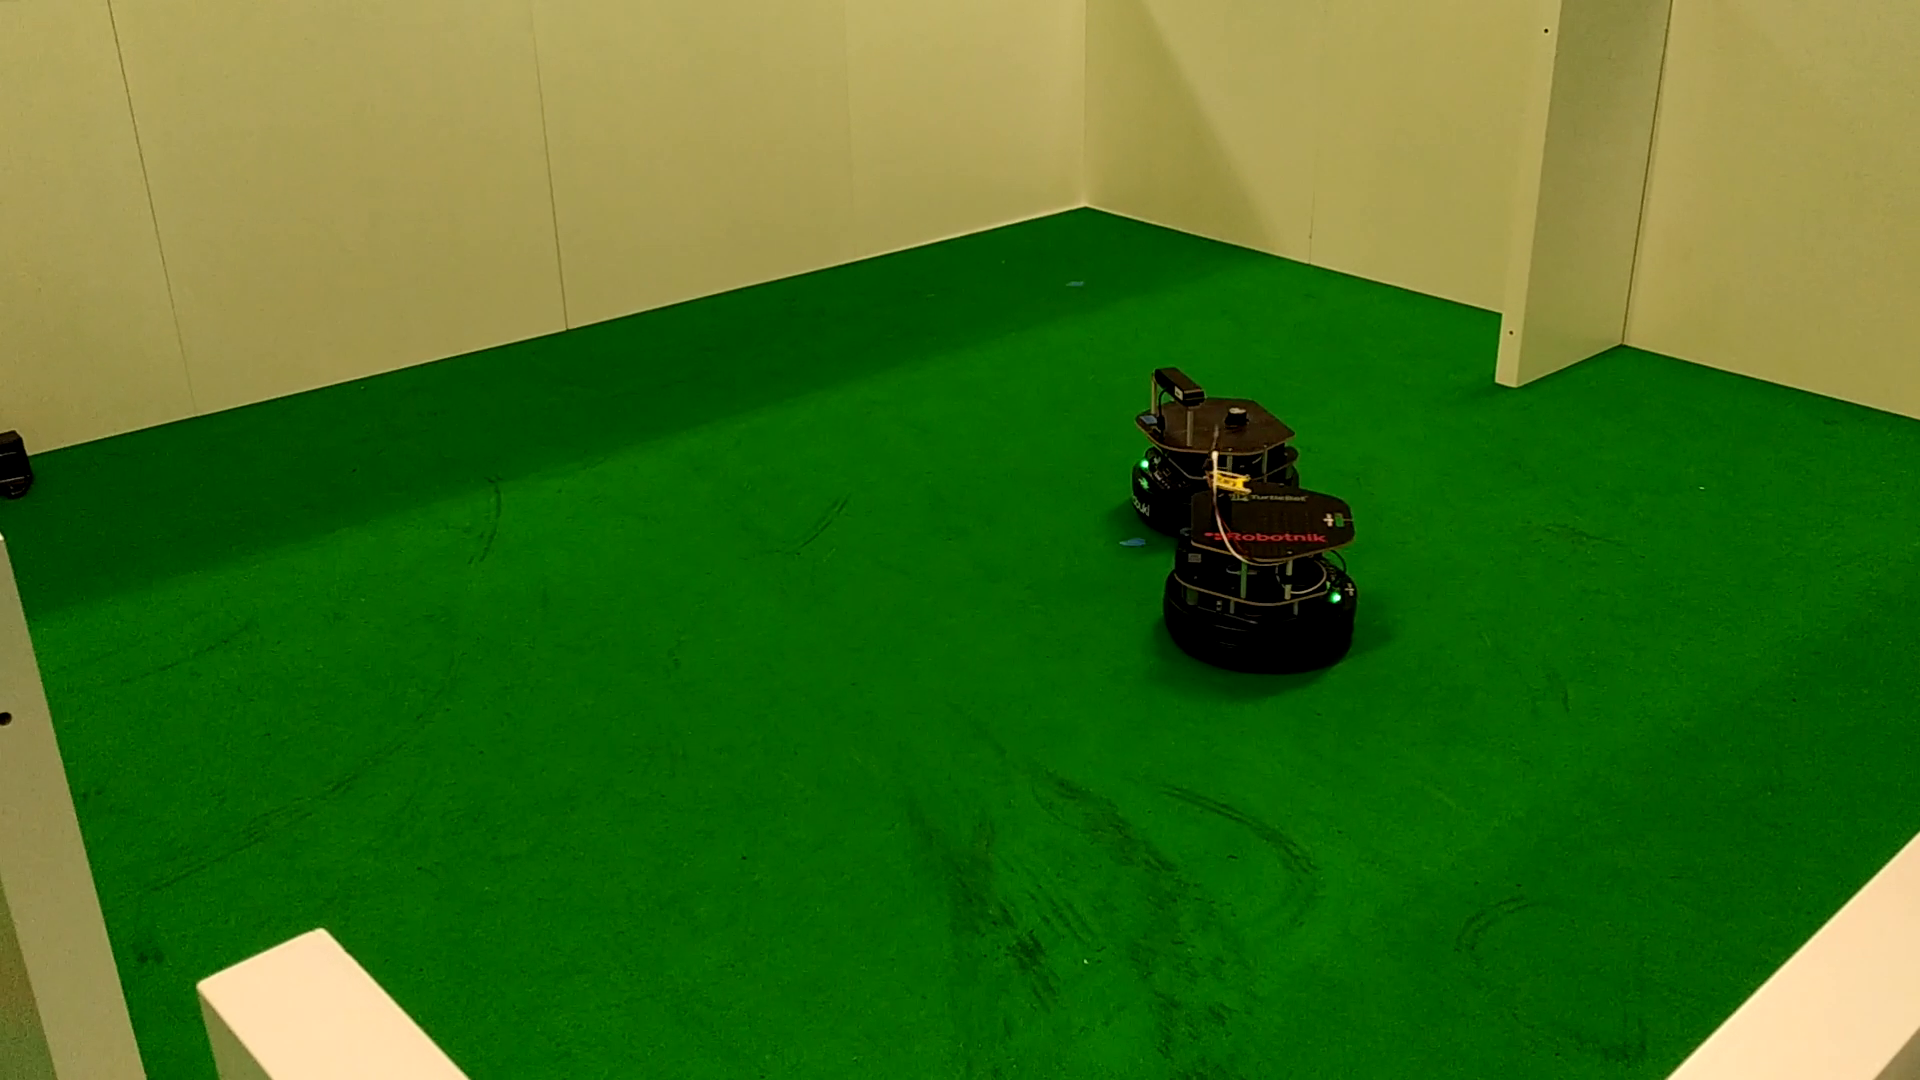
\includegraphics[width=\linewidth]{imgs/chapter5/exp3robot1.png}
     \caption{Robot avoiding dynamic robot 1}
     \label{fig::exp3robot1}
  \end{subfigure}
  \begin{subfigure}[b]{0.49\linewidth}
    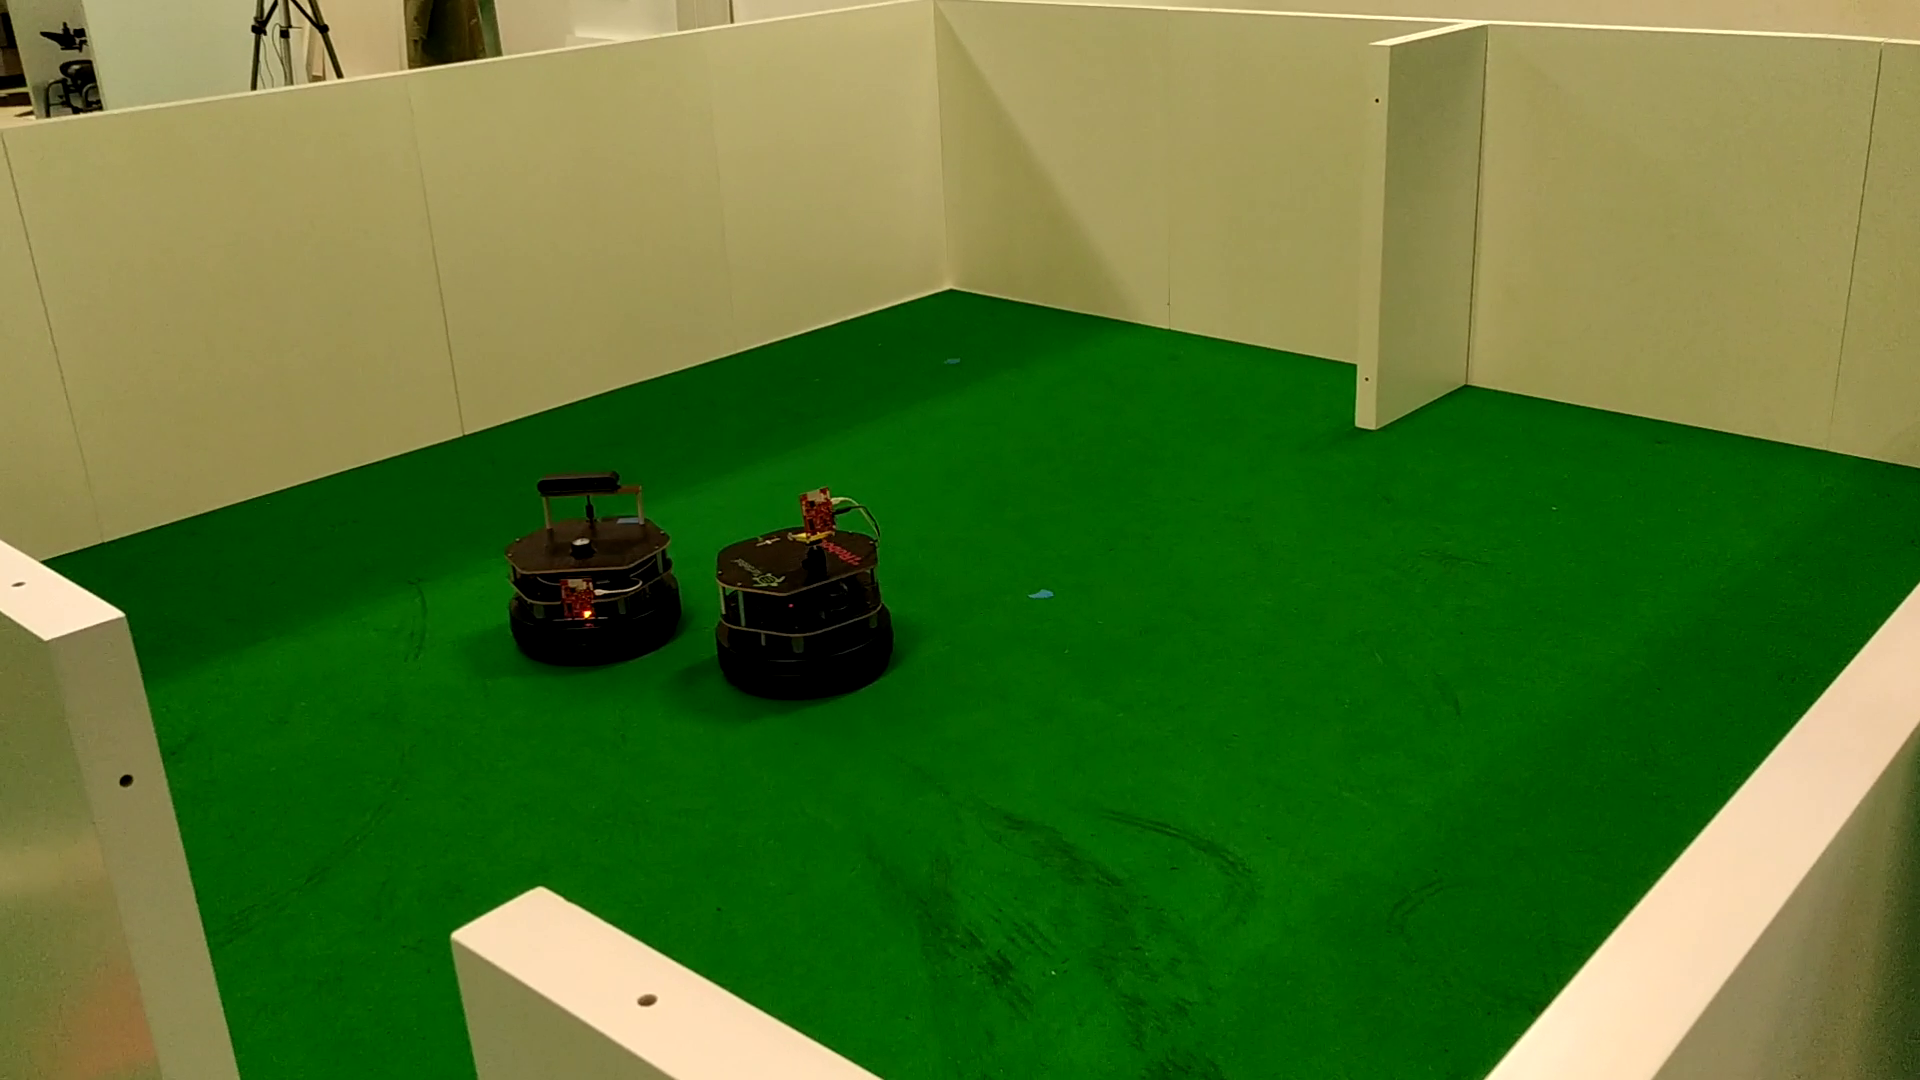
\includegraphics[width=\linewidth]{imgs/chapter5/exp3robot2.png}
    \caption{Robot avoiding dynamic robot 2}
    \label{fig::exp3robot2}
  \end{subfigure}
  \caption{Robot avoiding dynamic robot }
  \label{fig:exp3robot}
\end{figure}

However if the robot comes from behind there is the chance of it crashing because the radar as only a small field of view of 120º.
\subsection{Discussion}
The robot was able to handle dynamic obstacles using only the \ac{FMCW} \ac{radar}, this means that it might be feasible to only use this sensor for obstacle avoidance in ever changing indoor environments.

\section {Dynamic Obstacles in uncontrolled environment}
In the following test we want to answer two things: (1) Is the robot able to avoid people that obstruct its pre planned path only using the  \ac{FMCW} radar as an obstacle detector, and (2) if in this case it is also able to clear previously obstructed spaces (by the person in this case) by ray tracing its environment. This last requirement may provide to be difficult to get since the radar point cloud is less dense than the 2D laser range finder.

\subsection{Experimental Setup}
First a map was created of the \ac{IRIS} laboratory using the package \texttt{gmapping} provided by \ac{ROS} (Fig. \ref{fig:map}). Then using the map and the package \texttt{\ac{AMCL}} we ensure that the robot localization is fairly reasonable. After that we set up the robot to do a certain navigation task.
The robot starting position and goal were set as shown in Figure \ref{fig:setup} in the \ac{IRIS} laboratory. 

\begin{figure}[ht!]
\centerline{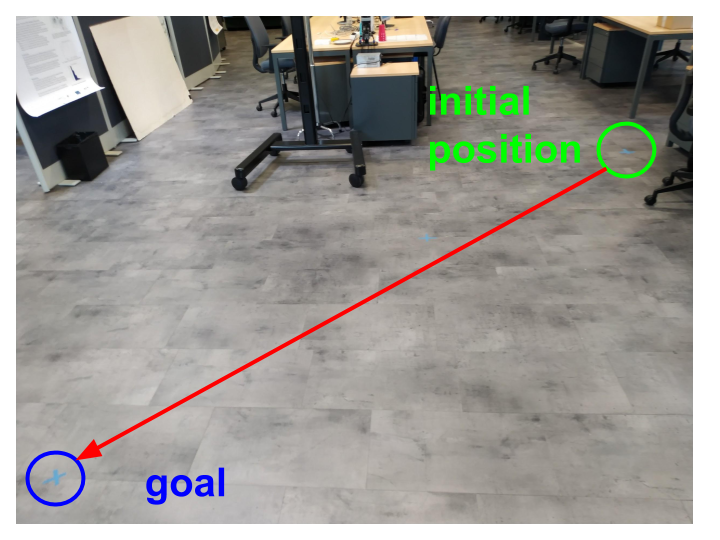
\includegraphics [width=0.8 \textwidth]{imgs/chapter5/setup.png}}
\caption[Experimental setup]{Experimental setup showing the initial position and the goal sent to the robot. A person will be put to obstruct the path of the robot}
\label{fig:setup}
\end{figure}


In this case a single person was instructed to actively obstruct the robot's forward movement until the robot reaches its first goal. After reaching it the person is removed from the environment  and the robot is  instantaneously given a second goal which in this case is its the starting position. 

\subsection{Results}
In the following sections we will describe how the robot behaved when under different type of sensor sources. With \ac{LiDAR}, \ac{FMCW} \ac{radar} and both.

\subsubsection*{\ac{LiDAR}}
As expected the robot was able to detect and avoid the person in all 5 cases. However it should be noted that in one of this cases the robot tried to avoid it by going through an obstructed space (that was not the person) due to a missed detection. This lead to collision. The robot was also able to clear the previously obstructed spaces, getting to the starting position without avoiding past marked obstacles.

\subsection*{\ac{FMCW} \ac{radar}}
The \ac{radar} was also able to detect the obstructing person and managed to plan around it in all cases as shown in Figures \ref{fig::radarperson1}, \ref{fig::radarperson2} and \ref{fig::radarperson3}. Since the radar cloud is less dense, clearing marked obstacles was slower than in the \ac{LiDAR} case. However this did not impact the overall performance of the navigation task in a significant way since it still went to the starting position in an almost straight line (Figure \ref{fig::radarperson4}).
\begin{figure}[h!]
  \centering
  \begin{subfigure}[b]{0.49\linewidth}
    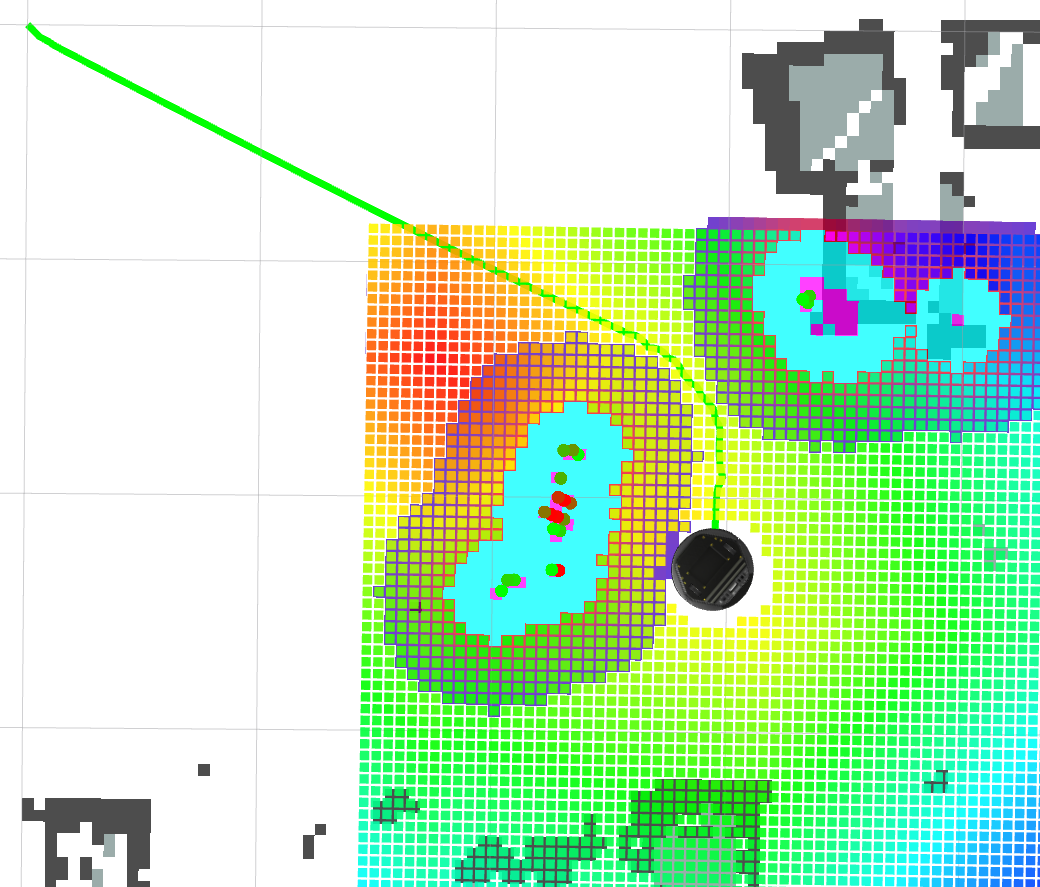
\includegraphics[width=\linewidth]{imgs/chapter5/radarperson1.png}
     \caption{Robot avoiding planning around the person blocking it}
     \label{fig::radarperson1}
  \end{subfigure}
  \begin{subfigure}[b]{0.49\linewidth}
    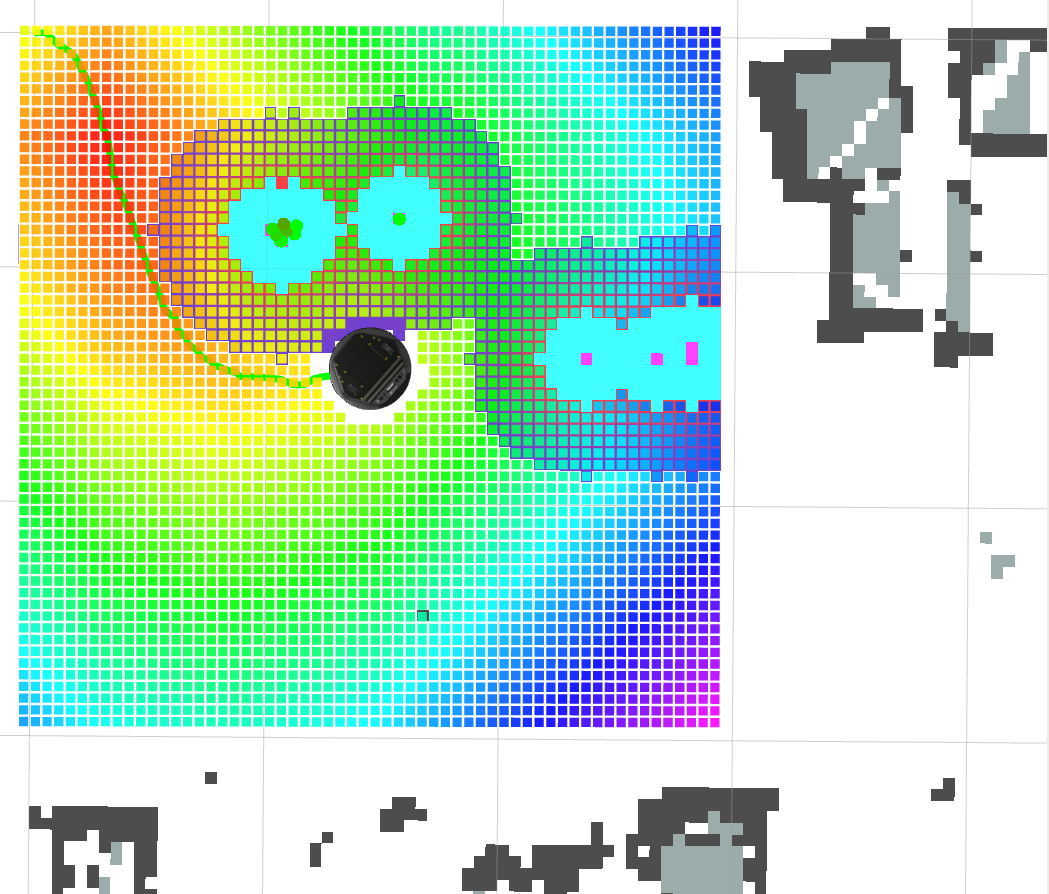
\includegraphics[width=\linewidth]{imgs/chapter5/radarperson2.png}
    \caption{Robot re planning around the person blocking it}
    \label{fig::radarperson2}
  \end{subfigure}
  \begin{subfigure}[b]{0.49\linewidth}
    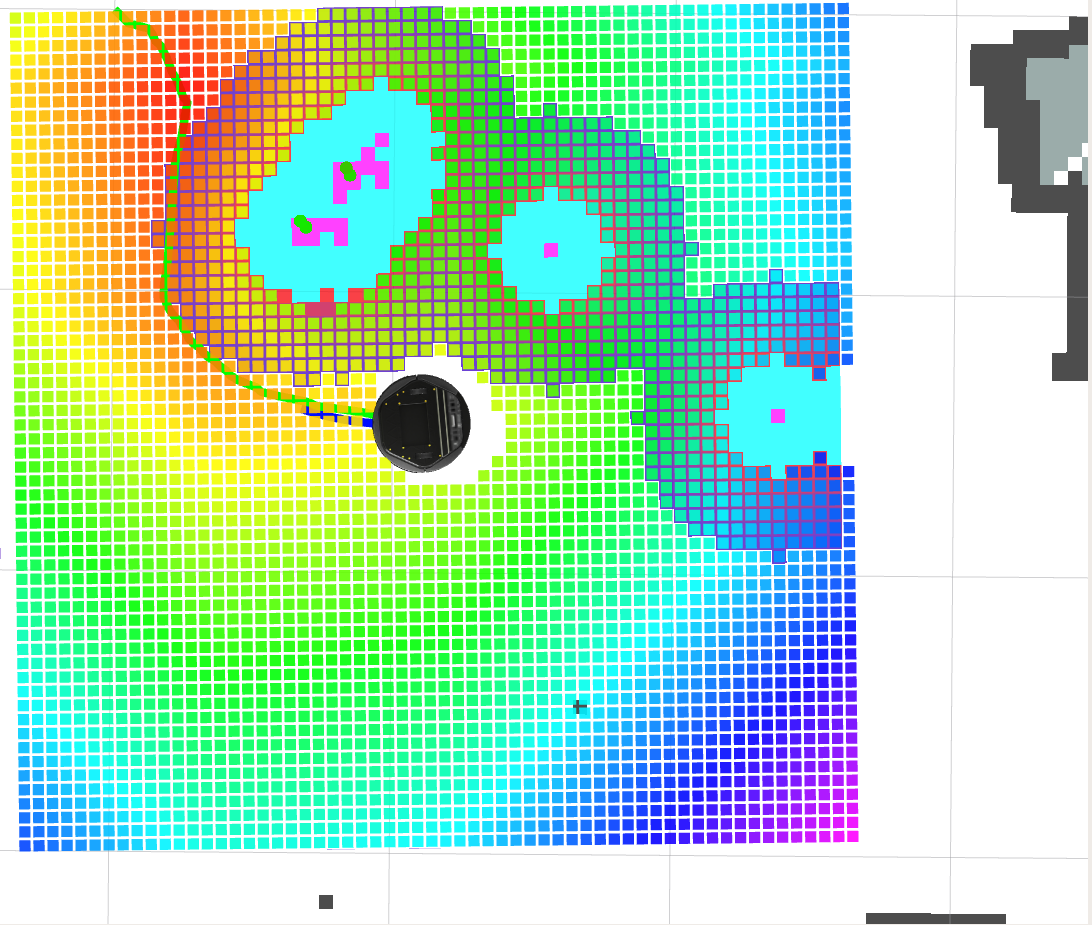
\includegraphics[width=\linewidth]{imgs/chapter5/radarperson3.png}
    \caption{Turtlebot stopping and adjust velocity to avoid person}
    \label{fig::radarperson3}
  \end{subfigure}
  \begin{subfigure}[b]{0.49\linewidth}
    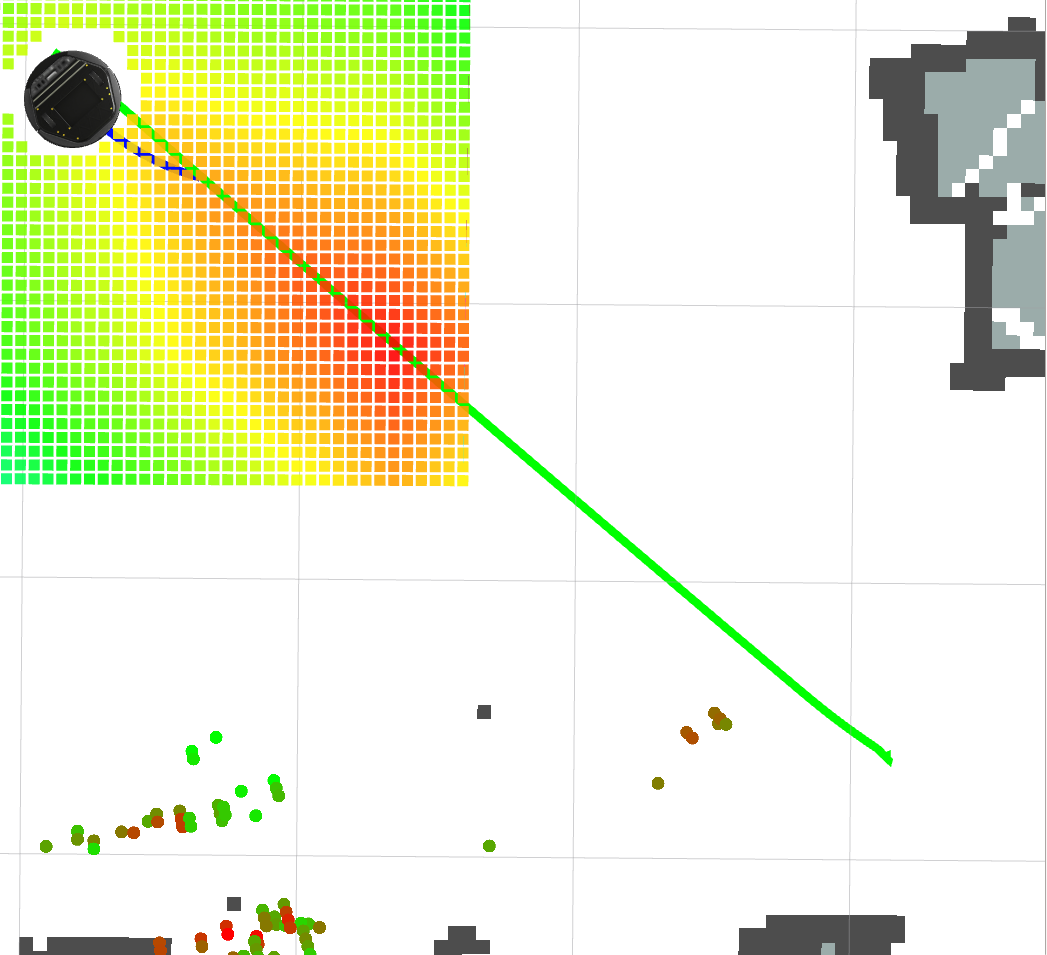
\includegraphics[width=\linewidth]{imgs/chapter5/radarperson4.png}
    \caption{Turtlebot returning to initial position in a straight line with no obstacles obstructing it}
    \label{fig::radarperson4}
  \end{subfigure}
\end{figure}
\subsection{Discussion}
 The \ac{FMCW} radar was able to perform 
obstacle avoidance of dynamic obstacles (in this case a person) that continuously obstructed its path at 5 different times in the same environment which may suggest the use of the \ac{FMCW} \ac{radar} as an alternate sensory unit over the \ac{LiDAR}.
